\documentclass[10pt,a4paper]{article}
\usepackage[T1]{fontenc}
\usepackage{lmodern,microtype,amsmath,amssymb,graphicx,booktabs,tabularx,array,longtable,xcolor,fancyhdr,titlesec}
\usepackage[margin=19mm,headheight=15pt,bottom=21mm]{geometry}
\usepackage[hidelinks,pdfauthor={},pdftitle={Three-Stage Thermoelectric Cooling of an HgCdTe Detector: Design and Thermal Performance}]{hyperref}
\pdfinfoomitdate=1\pdftrailerid{}\pdfsuppressptexinfo=15
\definecolor{navy}{HTML}{19334B}\definecolor{blue}{HTML}{3E7099}\definecolor{rust}{HTML}{A35437}
\hypersetup{colorlinks=true,linkcolor=navy,urlcolor=blue}
\pagestyle{fancy}\fancyhf{}\fancyhead[L]{\scriptsize HgCdTe DETECTOR | THERMAL AND ELECTRICAL ENGINEERING}\fancyhead[R]{\scriptsize 09 NOV 2026}
\fancyfoot[L]{\scriptsize Synthetic reference; not OEM-validated}\fancyfoot[R]{\scriptsize\thepage}
\setlength{\parindent}{0pt}\setlength{\parskip}{4pt}\setlength{\tabcolsep}{4pt}\renewcommand{\arraystretch}{1.12}
\setcounter{tocdepth}{1}
\widowpenalty=10000\clubpenalty=10000
\titleformat{\section}{\Large\bfseries\color{navy}}{\thesection}{.55em}{}
\newcommand{\fig}[4][.91]{\begin{figure}[!htbp]\centering\includegraphics[width=#1\linewidth]{figures/#2.#3}\caption{#4}\end{figure}}
% Frozen source-derived tables. Auto-generated; do not hand-edit.
\newcommand{\stagebudgetrows}{1 & 58 & 179.9602 & 614.7396 & 1.086948 & 262.732 \\
2 & 22 & 46.1636 & 176.5165 & 0.325882 & 81.390 \\
3 & 8 & 5.1576 & 43.7058 & 0.096371 & 24.642 \\}
\newcommand{\cavityrows}{Ceramic C1 & 1.15901 & 0.20874 & 1.36775 \\
Ceramic C2 & 1.44533 & 0.23389 & 1.67923 \\
Ceramic C3 & 1.06469 & 0.15770 & 1.22239 \\
Detector & 0.22352 & 0.02375 & 0.24726 \\
TOTAL & 3.89255 & 0.62408 & 4.51663 \\}
\newcommand{\operatingrows}{Detector temperature (K) & 209.987981 & 210.625214 \\
Terminal voltage (V) & 1.524071 & 1.522462 \\
Electrical input (W) & 0.609628 & 0.608985 \\
Bath rejection (W) & 0.590323 & 0.594044 \\
Pressure (Pa) & 0 (cavity off) & 100 (Kr) \\}
\newcommand{\nodetablerows}{Stage0 Hot & 303.65655 \\
Stage0 Cold & 265.90329 \\
Stage1 Hot & 266.34287 \\
Stage1 Cold & 236.00259 \\
Stage2 Hot & 236.15716 \\
Stage2 Cold & 210.52765 \\
Carrier & 210.55066 \\
Die & 210.62521 \\}
\newcommand{\iterationrows}{1 & 210.599377 & 1.690e-02 & 3.914e-15 \\
2 & 210.624173 & 2.066e-03 & 4.580e-16 \\
3 & 210.625110 & 4.135e-04 & 1.478e-15 \\
4 & 210.625220 & 8.254e-05 & 2.928e-15 \\
5 & 210.625214 & 1.653e-05 & 5.503e-15 \\}
\newcommand{\residualrows}{Global energy & 8.8674e-09 & W \\
Worst stage balance & 4.9061e-09 & W \\
Ceramic pad heat & 5.5025e-15 & W \\
Worst individual leg & 1.2364e-13 & W \\
Final pad temperature change & 1.6535e-05 & K \\}
\newcommand{\materialrows}{40 & 31.477086 & 1.226120 & 2.776424 & -39.762194 & 0.837035 & 3.928920 \\
60 & 44.991486 & 1.550968 & 2.488935 & -53.616397 & 1.156199 & 3.246955 \\
80 & 60.679339 & 1.955036 & 2.260290 & -67.469437 & 1.522950 & 2.816874 \\
100 & 77.996604 & 2.446265 & 2.072406 & -81.936140 & 1.920207 & 2.536709 \\
120 & 96.944423 & 3.004830 & 1.909416 & -95.992742 & 2.354830 & 2.310364 \\
140 & 115.755946 & 3.567364 & 1.764537 & -109.847998 & 2.820018 & 2.129254 \\
160 & 133.684757 & 4.343818 & 1.630978 & -122.547039 & 3.319204 & 1.973635 \\
180 & 150.458980 & 5.175731 & 1.515526 & -134.499967 & 3.835302 & 1.851971 \\
200 & 166.078757 & 6.067058 & 1.415926 & -145.840430 & 4.371811 & 1.744414 \\
220 & 179.321421 & 7.073284 & 1.332165 & -156.231255 & 4.932113 & 1.653884 \\
240 & 190.594863 & 8.138932 & 1.257469 & -165.737958 & 5.570441 & 1.574639 \\
260 & 199.219885 & 9.351143 & 1.194083 & -174.568277 & 6.232621 & 1.506729 \\
280 & 205.739245 & 10.694094 & 1.137484 & -182.445326 & 6.884545 & 1.447332 \\
300 & 212.462550 & 12.080611 & 1.099006 & -189.575244 & 7.543277 & 1.399227 \\}
\newcommand{\legrows}{0 & 0 & N & -2.030000 & -2.030000 \\
1 & 0 & P & -1.450000 & -2.030000 \\
2 & 0 & N & -0.870000 & -2.030000 \\
3 & 0 & P & -0.290000 & -2.030000 \\
4 & 0 & N & 0.290000 & -2.030000 \\
5 & 0 & P & 0.870000 & -2.030000 \\
6 & 0 & N & 1.450000 & -2.030000 \\
7 & 0 & P & 2.030000 & -2.030000 \\
8 & 0 & N & 2.030000 & -1.450000 \\
9 & 0 & P & 1.450000 & -1.450000 \\
10 & 0 & N & 0.870000 & -1.450000 \\
11 & 0 & P & 0.290000 & -1.450000 \\
12 & 0 & N & -0.290000 & -1.450000 \\
13 & 0 & P & -0.870000 & -1.450000 \\
14 & 0 & N & -1.450000 & -1.450000 \\
15 & 0 & P & -2.030000 & -1.450000 \\
16 & 0 & N & -2.030000 & -0.870000 \\
17 & 0 & P & -1.450000 & -0.870000 \\
18 & 0 & N & -0.870000 & -0.870000 \\
19 & 0 & P & -0.290000 & -0.870000 \\
20 & 0 & N & 0.290000 & -0.870000 \\
21 & 0 & P & 0.870000 & -0.870000 \\
22 & 0 & N & 1.450000 & -0.870000 \\
23 & 0 & P & 2.030000 & -0.870000 \\
24 & 0 & N & 2.030000 & -0.290000 \\
25 & 0 & P & 1.450000 & -0.290000 \\
26 & 0 & N & 0.870000 & -0.290000 \\
27 & 0 & P & 0.290000 & -0.290000 \\
28 & 0 & N & -0.290000 & -0.290000 \\
29 & 0 & P & -0.870000 & -0.290000 \\
30 & 0 & N & -1.450000 & -0.290000 \\
31 & 0 & P & -2.030000 & -0.290000 \\
32 & 0 & N & -2.030000 & 0.290000 \\
33 & 0 & P & -1.450000 & 0.290000 \\
34 & 0 & N & -0.870000 & 0.290000 \\
35 & 0 & P & -0.290000 & 0.290000 \\
36 & 0 & N & 0.290000 & 0.290000 \\
37 & 0 & P & 0.870000 & 0.290000 \\
38 & 0 & N & 1.450000 & 0.290000 \\
39 & 0 & P & 2.030000 & 0.290000 \\
40 & 0 & N & 2.030000 & 0.870000 \\
41 & 0 & P & 1.450000 & 0.870000 \\
42 & 0 & N & 0.870000 & 0.870000 \\
43 & 0 & P & 0.290000 & 0.870000 \\
44 & 0 & N & -0.290000 & 0.870000 \\
45 & 0 & P & -0.870000 & 0.870000 \\
46 & 0 & N & -1.450000 & 0.870000 \\
47 & 0 & P & -2.030000 & 0.870000 \\
48 & 0 & N & -2.030000 & 1.450000 \\
49 & 0 & P & -1.450000 & 1.450000 \\
50 & 0 & N & -0.870000 & 1.450000 \\
51 & 0 & P & -0.290000 & 1.450000 \\
52 & 0 & N & 0.290000 & 1.450000 \\
53 & 0 & P & 0.870000 & 1.450000 \\
54 & 0 & N & 1.450000 & 1.450000 \\
55 & 0 & P & 2.030000 & 1.450000 \\
56 & 0 & N & 2.030000 & 2.030000 \\
57 & 0 & P & 1.450000 & 2.030000 \\
58 & 1 & N & 1.450000 & 0.870000 \\
59 & 1 & P & 0.870000 & 0.870000 \\
60 & 1 & N & 0.290000 & 0.870000 \\
61 & 1 & P & -0.290000 & 0.870000 \\
62 & 1 & N & -0.870000 & 0.870000 \\
63 & 1 & P & -1.450000 & 0.870000 \\
64 & 1 & N & -1.450000 & 0.290000 \\
65 & 1 & P & -0.870000 & 0.290000 \\
66 & 1 & N & -0.290000 & 0.290000 \\
67 & 1 & P & 0.290000 & 0.290000 \\
68 & 1 & N & 0.870000 & 0.290000 \\
69 & 1 & P & 1.450000 & 0.290000 \\
70 & 1 & N & 1.450000 & -0.290000 \\
71 & 1 & P & 0.870000 & -0.290000 \\
72 & 1 & N & 0.290000 & -0.290000 \\
73 & 1 & P & -0.290000 & -0.290000 \\
74 & 1 & N & -0.870000 & -0.290000 \\
75 & 1 & P & -1.450000 & -0.290000 \\
76 & 1 & N & -1.450000 & -0.870000 \\
77 & 1 & P & -0.870000 & -0.870000 \\
78 & 1 & N & -0.290000 & -0.870000 \\
79 & 1 & P & 0.290000 & -0.870000 \\
80 & 2 & N & 0.870000 & -0.290000 \\
81 & 2 & P & 0.290000 & -0.290000 \\
82 & 2 & N & -0.290000 & -0.290000 \\
83 & 2 & P & -0.870000 & -0.290000 \\
84 & 2 & N & -0.870000 & 0.290000 \\
85 & 2 & P & -0.290000 & 0.290000 \\
86 & 2 & N & 0.290000 & 0.290000 \\
87 & 2 & P & 0.870000 & 0.290000 \\}
\newcommand{\padrows}{0 & 6 & 0.000000 & 0.000000 & 1.584250 & 37.21000000 & -5.9404375264e-01 \\
0 & 8 & -2.030000 & -2.415000 & 2.084250 & 0.58100000 & +6.9212449542e-03 \\
0 & 9 & -1.160000 & -2.030000 & 2.084250 & 0.54000000 & +2.1001118011e-02 \\
0 & 10 & -0.000000 & -2.030000 & 2.084250 & 0.54000000 & +2.0799385661e-02 \\
0 & 11 & -2.030000 & -1.160000 & 2.084250 & 0.54000000 & +2.1333430585e-02 \\
0 & 12 & -1.160000 & -1.450000 & 2.084250 & 0.54000000 & +2.0925106301e-02 \\
0 & 13 & -1.160000 & -0.870000 & 2.084250 & 0.54000000 & +2.1098181465e-02 \\
0 & 14 & -2.030000 & -0.000000 & 2.084250 & 0.54000000 & +2.1661444954e-02 \\
0 & 15 & -1.160000 & -0.290000 & 2.084250 & 0.54000000 & +2.1280527762e-02 \\
0 & 16 & -0.000000 & -1.450000 & 2.084250 & 0.54000000 & +2.0726535211e-02 \\
0 & 17 & 0.000000 & -0.870000 & 2.084250 & 0.54000000 & +2.0872339885e-02 \\
0 & 18 & -0.000000 & -0.290000 & 2.084250 & 0.54000000 & +2.1135046258e-02 \\
0 & 19 & 1.160000 & -2.030000 & 2.084250 & 0.54000000 & +2.0762274895e-02 \\
0 & 20 & 2.030000 & -1.740000 & 2.084250 & 0.54000000 & +2.0894962316e-02 \\
0 & 21 & 1.160000 & -1.450000 & 2.084250 & 0.54000000 & +2.0664089207e-02 \\
0 & 22 & 1.160000 & -0.870000 & 2.084250 & 0.54000000 & +2.0730610371e-02 \\
0 & 23 & 1.160000 & -0.290000 & 2.084250 & 0.54000000 & +2.0987932670e-02 \\
0 & 24 & 2.030000 & -0.580000 & 2.084250 & 0.54000000 & +2.1025501033e-02 \\
0 & 25 & -1.160000 & 0.290000 & 2.084250 & 0.54000000 & +2.1501510390e-02 \\
0 & 26 & -2.030000 & 1.160000 & 2.084250 & 0.54000000 & +2.2056807823e-02 \\
0 & 27 & -1.160000 & 0.870000 & 2.084250 & 0.54000000 & +2.1665224003e-02 \\
0 & 28 & -1.160000 & 1.450000 & 2.084250 & 0.54000000 & +2.1972015528e-02 \\
0 & 29 & 0.000000 & 0.290000 & 2.084250 & 0.54000000 & +2.1329922044e-02 \\
0 & 30 & -0.000000 & 0.870000 & 2.084250 & 0.54000000 & +2.1513476612e-02 \\
0 & 31 & 0.000000 & 1.450000 & 2.084250 & 0.54000000 & +2.1762448001e-02 \\
0 & 32 & 1.160000 & 0.290000 & 2.084250 & 0.54000000 & +2.1132384800e-02 \\
0 & 33 & 2.030000 & 0.580000 & 2.084250 & 0.54000000 & +2.1315494607e-02 \\
0 & 34 & 1.160000 & 0.870000 & 2.084250 & 0.54000000 & +2.1316483722e-02 \\
0 & 35 & 1.160000 & 1.450000 & 2.084250 & 0.54000000 & +2.1497446937e-02 \\
0 & 36 & 0.088570 & 2.858995 & 2.084250 & 0.67225000 & -2.2200926469e-02 \\
0 & 37 & 2.030000 & 1.740000 & 2.084250 & 0.54000000 & +2.1652376653e-02 \\
0 & 38 & 1.450000 & 2.379622 & 2.084250 & 0.51850000 & +1.4709356454e-02 \\
1 & 44 & -1.740000 & -2.030000 & 2.684250 & 0.54000000 & -6.1717204457e-03 \\
1 & 45 & -0.580000 & -2.030000 & 2.684250 & 0.54000000 & -5.7923394592e-03 \\
1 & 46 & 0.580000 & -2.030000 & 2.684250 & 0.54000000 & -5.6313481447e-03 \\
1 & 47 & -1.740000 & -1.450000 & 2.684250 & 0.54000000 & -5.8945158835e-03 \\
1 & 48 & -1.740000 & -0.870000 & 2.684250 & 0.54000000 & -6.1272498337e-03 \\
1 & 49 & -0.580000 & -1.450000 & 2.684250 & 0.54000000 & -5.6677985879e-03 \\
1 & 50 & -0.580000 & -0.870000 & 2.684250 & 0.54000000 & -5.9073535857e-03 \\
1 & 51 & -1.740000 & -0.290000 & 2.684250 & 0.54000000 & -6.2861601984e-03 \\
1 & 52 & -1.740000 & 0.290000 & 2.684250 & 0.54000000 & -6.4929448577e-03 \\
1 & 53 & -0.580000 & -0.290000 & 2.684250 & 0.54000000 & -6.1441766581e-03 \\
1 & 54 & 0.580000 & -1.450000 & 2.684250 & 0.54000000 & -5.4949366062e-03 \\
1 & 55 & 0.580000 & -0.870000 & 2.684250 & 0.54000000 & -5.6165637076e-03 \\
1 & 56 & 0.580000 & -0.290000 & 2.684250 & 0.54000000 & -5.9284010470e-03 \\
1 & 57 & 1.740000 & -2.030000 & 2.684250 & 0.54000000 & -5.5964450493e-03 \\
1 & 58 & 1.740000 & -1.450000 & 2.684250 & 0.54000000 & -5.5750930796e-03 \\
1 & 59 & 1.740000 & -0.870000 & 2.684250 & 0.54000000 & -5.5316729855e-03 \\
1 & 60 & 1.740000 & -0.290000 & 2.684250 & 0.54000000 & -5.7862099653e-03 \\
1 & 61 & -0.580000 & 0.290000 & 2.684250 & 0.54000000 & -6.4257386885e-03 \\
1 & 62 & -1.740000 & 0.870000 & 2.684250 & 0.54000000 & -6.8576261766e-03 \\
1 & 63 & -1.740000 & 1.450000 & 2.684250 & 0.54000000 & -7.0890067759e-03 \\
1 & 64 & -0.580000 & 0.870000 & 2.684250 & 0.54000000 & -6.6249732312e-03 \\
1 & 65 & -0.580000 & 1.450000 & 2.684250 & 0.54000000 & -7.0137372522e-03 \\
1 & 66 & 0.580000 & 0.290000 & 2.684250 & 0.54000000 & -6.1746390641e-03 \\
1 & 67 & 0.580000 & 0.870000 & 2.684250 & 0.54000000 & -6.3948651910e-03 \\
1 & 68 & 0.580000 & 1.450000 & 2.684250 & 0.54000000 & -6.7126784447e-03 \\
1 & 69 & 1.740000 & 0.290000 & 2.684250 & 0.54000000 & -6.0016216656e-03 \\
1 & 70 & 1.740000 & 0.870000 & 2.684250 & 0.54000000 & -6.1198269805e-03 \\
1 & 71 & 1.740000 & 1.450000 & 2.684250 & 0.54000000 & -6.5247521871e-03 \\
1 & 72 & 1.740000 & 2.030000 & 2.684250 & 0.54000000 & -6.8707555753e-03 \\
1 & 74 & 0.870000 & 2.300000 & 3.184250 & 0.12000000 & +2.3941388903e-05 \\
1 & 75 & 1.450000 & 1.470862 & 3.184250 & 0.67900000 & +5.1504788556e-03 \\
1 & 76 & -1.450000 & -0.580000 & 3.184250 & 0.54000000 & +1.6210670281e-02 \\
1 & 77 & -0.580000 & -0.870000 & 3.184250 & 0.54000000 & +1.6207954022e-02 \\
1 & 78 & -0.580000 & -0.290000 & 3.184250 & 0.54000000 & +1.6071664242e-02 \\
1 & 79 & 0.290000 & -1.435162 & 3.184250 & 0.65650000 & +1.1539642240e-02 \\
1 & 80 & 0.580000 & -0.290000 & 3.184250 & 0.54000000 & +1.6217492734e-02 \\
1 & 81 & 1.450000 & 0.000000 & 3.184250 & 0.54000000 & +1.6376311378e-02 \\
1 & 82 & -1.450000 & 0.580000 & 3.184250 & 0.54000000 & +1.6153119097e-02 \\
1 & 83 & -0.580000 & 0.290000 & 3.184250 & 0.54000000 & +1.6048683270e-02 \\
1 & 84 & -0.580000 & 0.870000 & 3.184250 & 0.54000000 & +1.6098735692e-02 \\
1 & 85 & 0.580000 & 0.290000 & 3.184250 & 0.54000000 & +1.6138044094e-02 \\
1 & 86 & 0.580000 & 0.870000 & 3.184250 & 0.54000000 & +1.6218414034e-02 \\
2 & 92 & -1.160000 & -0.870000 & 3.784250 & 0.54000000 & -4.1229763184e-03 \\
2 & 93 & -1.160000 & -0.290000 & 3.784250 & 0.54000000 & -4.0325885849e-03 \\
2 & 94 & 0.000000 & -0.870000 & 3.784250 & 0.54000000 & -4.3372223253e-03 \\
2 & 95 & -0.000000 & -0.290000 & 3.784250 & 0.54000000 & -4.1255544021e-03 \\
2 & 96 & 1.160000 & -0.290000 & 3.784250 & 0.54000000 & -4.2477066490e-03 \\
2 & 97 & -1.160000 & 0.290000 & 3.784250 & 0.54000000 & -3.9991911145e-03 \\
2 & 98 & -1.160000 & 0.870000 & 3.784250 & 0.54000000 & -4.0132490723e-03 \\
2 & 99 & 0.000000 & 0.290000 & 3.784250 & 0.54000000 & -4.0452781812e-03 \\
2 & 100 & 1.160000 & 0.290000 & 3.784250 & 0.54000000 & -4.1617896577e-03 \\
2 & 101 & -0.000000 & 0.870000 & 3.784250 & 0.54000000 & -4.1215621922e-03 \\
2 & 102 & 1.160000 & 0.870000 & 3.784250 & 0.54000000 & -4.3855401752e-03 \\
2 & 104 & 0.870000 & 0.829062 & 4.284250 & 0.64000000 & +8.5720985048e-03 \\
2 & 105 & 0.692720 & -0.929413 & 4.284250 & 0.81350000 & +3.2580848072e-03 \\
2 & 106 & -0.000000 & -0.290000 & 4.284250 & 0.54000000 & +1.1238504436e-02 \\
2 & 107 & -0.870000 & 0.000000 & 4.284250 & 0.54000000 & +1.1290111066e-02 \\
2 & 108 & 0.000000 & 0.290000 & 4.284250 & 0.54000000 & +1.1233859859e-02 \\
3 & 114 & 0.580000 & 0.290000 & 4.884250 & 0.54000000 & -1.2327805666e-03 \\
3 & 115 & -0.580000 & -0.290000 & 4.884250 & 0.54000000 & -1.2229792254e-03 \\
3 & 116 & 0.580000 & -0.290000 & 4.884250 & 0.54000000 & -1.2662612022e-03 \\
3 & 117 & -0.580000 & 0.290000 & 4.884250 & 0.54000000 & -1.2279447029e-03 \\
3 & 119 & -0.000000 & -0.000000 & 5.384250 & 4.41000000 & +4.9499656971e-03 \\}

\newcommand{\legrowsA}{0 & 0 & N & -2.030000 & -2.030000 \\
1 & 0 & P & -1.450000 & -2.030000 \\
2 & 0 & N & -0.870000 & -2.030000 \\
3 & 0 & P & -0.290000 & -2.030000 \\
4 & 0 & N & 0.290000 & -2.030000 \\
5 & 0 & P & 0.870000 & -2.030000 \\
6 & 0 & N & 1.450000 & -2.030000 \\
7 & 0 & P & 2.030000 & -2.030000 \\
8 & 0 & N & 2.030000 & -1.450000 \\
9 & 0 & P & 1.450000 & -1.450000 \\
10 & 0 & N & 0.870000 & -1.450000 \\
11 & 0 & P & 0.290000 & -1.450000 \\
12 & 0 & N & -0.290000 & -1.450000 \\
13 & 0 & P & -0.870000 & -1.450000 \\
14 & 0 & N & -1.450000 & -1.450000 \\
15 & 0 & P & -2.030000 & -1.450000 \\
16 & 0 & N & -2.030000 & -0.870000 \\
17 & 0 & P & -1.450000 & -0.870000 \\
18 & 0 & N & -0.870000 & -0.870000 \\
19 & 0 & P & -0.290000 & -0.870000 \\
20 & 0 & N & 0.290000 & -0.870000 \\
21 & 0 & P & 0.870000 & -0.870000 \\
22 & 0 & N & 1.450000 & -0.870000 \\
23 & 0 & P & 2.030000 & -0.870000 \\
24 & 0 & N & 2.030000 & -0.290000 \\
25 & 0 & P & 1.450000 & -0.290000 \\
26 & 0 & N & 0.870000 & -0.290000 \\
27 & 0 & P & 0.290000 & -0.290000 \\
28 & 0 & N & -0.290000 & -0.290000 \\
29 & 0 & P & -0.870000 & -0.290000 \\
30 & 0 & N & -1.450000 & -0.290000 \\
31 & 0 & P & -2.030000 & -0.290000 \\
32 & 0 & N & -2.030000 & 0.290000 \\
33 & 0 & P & -1.450000 & 0.290000 \\
34 & 0 & N & -0.870000 & 0.290000 \\
35 & 0 & P & -0.290000 & 0.290000 \\
36 & 0 & N & 0.290000 & 0.290000 \\
37 & 0 & P & 0.870000 & 0.290000 \\
38 & 0 & N & 1.450000 & 0.290000 \\
39 & 0 & P & 2.030000 & 0.290000 \\
40 & 0 & N & 2.030000 & 0.870000 \\
41 & 0 & P & 1.450000 & 0.870000 \\
42 & 0 & N & 0.870000 & 0.870000 \\
43 & 0 & P & 0.290000 & 0.870000 \\}
\newcommand{\legrowsB}{44 & 0 & N & -0.290000 & 0.870000 \\
45 & 0 & P & -0.870000 & 0.870000 \\
46 & 0 & N & -1.450000 & 0.870000 \\
47 & 0 & P & -2.030000 & 0.870000 \\
48 & 0 & N & -2.030000 & 1.450000 \\
49 & 0 & P & -1.450000 & 1.450000 \\
50 & 0 & N & -0.870000 & 1.450000 \\
51 & 0 & P & -0.290000 & 1.450000 \\
52 & 0 & N & 0.290000 & 1.450000 \\
53 & 0 & P & 0.870000 & 1.450000 \\
54 & 0 & N & 1.450000 & 1.450000 \\
55 & 0 & P & 2.030000 & 1.450000 \\
56 & 0 & N & 2.030000 & 2.030000 \\
57 & 0 & P & 1.450000 & 2.030000 \\
58 & 1 & N & 1.450000 & 0.870000 \\
59 & 1 & P & 0.870000 & 0.870000 \\
60 & 1 & N & 0.290000 & 0.870000 \\
61 & 1 & P & -0.290000 & 0.870000 \\
62 & 1 & N & -0.870000 & 0.870000 \\
63 & 1 & P & -1.450000 & 0.870000 \\
64 & 1 & N & -1.450000 & 0.290000 \\
65 & 1 & P & -0.870000 & 0.290000 \\
66 & 1 & N & -0.290000 & 0.290000 \\
67 & 1 & P & 0.290000 & 0.290000 \\
68 & 1 & N & 0.870000 & 0.290000 \\
69 & 1 & P & 1.450000 & 0.290000 \\
70 & 1 & N & 1.450000 & -0.290000 \\
71 & 1 & P & 0.870000 & -0.290000 \\
72 & 1 & N & 0.290000 & -0.290000 \\
73 & 1 & P & -0.290000 & -0.290000 \\
74 & 1 & N & -0.870000 & -0.290000 \\
75 & 1 & P & -1.450000 & -0.290000 \\
76 & 1 & N & -1.450000 & -0.870000 \\
77 & 1 & P & -0.870000 & -0.870000 \\
78 & 1 & N & -0.290000 & -0.870000 \\
79 & 1 & P & 0.290000 & -0.870000 \\
80 & 2 & N & 0.870000 & -0.290000 \\
81 & 2 & P & 0.290000 & -0.290000 \\
82 & 2 & N & -0.290000 & -0.290000 \\
83 & 2 & P & -0.870000 & -0.290000 \\
84 & 2 & N & -0.870000 & 0.290000 \\
85 & 2 & P & -0.290000 & 0.290000 \\
86 & 2 & N & 0.290000 & 0.290000 \\
87 & 2 & P & 0.870000 & 0.290000 \\}

\newcommand{\legpairrows}{0 & 0 & N & -2.030000 & -2.030000 & 44 & 0 & N & -0.290000 & 0.870000 \\
1 & 0 & P & -1.450000 & -2.030000 & 45 & 0 & P & -0.870000 & 0.870000 \\
2 & 0 & N & -0.870000 & -2.030000 & 46 & 0 & N & -1.450000 & 0.870000 \\
3 & 0 & P & -0.290000 & -2.030000 & 47 & 0 & P & -2.030000 & 0.870000 \\
4 & 0 & N & 0.290000 & -2.030000 & 48 & 0 & N & -2.030000 & 1.450000 \\
5 & 0 & P & 0.870000 & -2.030000 & 49 & 0 & P & -1.450000 & 1.450000 \\
6 & 0 & N & 1.450000 & -2.030000 & 50 & 0 & N & -0.870000 & 1.450000 \\
7 & 0 & P & 2.030000 & -2.030000 & 51 & 0 & P & -0.290000 & 1.450000 \\
8 & 0 & N & 2.030000 & -1.450000 & 52 & 0 & N & 0.290000 & 1.450000 \\
9 & 0 & P & 1.450000 & -1.450000 & 53 & 0 & P & 0.870000 & 1.450000 \\
10 & 0 & N & 0.870000 & -1.450000 & 54 & 0 & N & 1.450000 & 1.450000 \\
11 & 0 & P & 0.290000 & -1.450000 & 55 & 0 & P & 2.030000 & 1.450000 \\
12 & 0 & N & -0.290000 & -1.450000 & 56 & 0 & N & 2.030000 & 2.030000 \\
13 & 0 & P & -0.870000 & -1.450000 & 57 & 0 & P & 1.450000 & 2.030000 \\
14 & 0 & N & -1.450000 & -1.450000 & 58 & 1 & N & 1.450000 & 0.870000 \\
15 & 0 & P & -2.030000 & -1.450000 & 59 & 1 & P & 0.870000 & 0.870000 \\
16 & 0 & N & -2.030000 & -0.870000 & 60 & 1 & N & 0.290000 & 0.870000 \\
17 & 0 & P & -1.450000 & -0.870000 & 61 & 1 & P & -0.290000 & 0.870000 \\
18 & 0 & N & -0.870000 & -0.870000 & 62 & 1 & N & -0.870000 & 0.870000 \\
19 & 0 & P & -0.290000 & -0.870000 & 63 & 1 & P & -1.450000 & 0.870000 \\
20 & 0 & N & 0.290000 & -0.870000 & 64 & 1 & N & -1.450000 & 0.290000 \\
21 & 0 & P & 0.870000 & -0.870000 & 65 & 1 & P & -0.870000 & 0.290000 \\
22 & 0 & N & 1.450000 & -0.870000 & 66 & 1 & N & -0.290000 & 0.290000 \\
23 & 0 & P & 2.030000 & -0.870000 & 67 & 1 & P & 0.290000 & 0.290000 \\
24 & 0 & N & 2.030000 & -0.290000 & 68 & 1 & N & 0.870000 & 0.290000 \\
25 & 0 & P & 1.450000 & -0.290000 & 69 & 1 & P & 1.450000 & 0.290000 \\
26 & 0 & N & 0.870000 & -0.290000 & 70 & 1 & N & 1.450000 & -0.290000 \\
27 & 0 & P & 0.290000 & -0.290000 & 71 & 1 & P & 0.870000 & -0.290000 \\
28 & 0 & N & -0.290000 & -0.290000 & 72 & 1 & N & 0.290000 & -0.290000 \\
29 & 0 & P & -0.870000 & -0.290000 & 73 & 1 & P & -0.290000 & -0.290000 \\
30 & 0 & N & -1.450000 & -0.290000 & 74 & 1 & N & -0.870000 & -0.290000 \\
31 & 0 & P & -2.030000 & -0.290000 & 75 & 1 & P & -1.450000 & -0.290000 \\
32 & 0 & N & -2.030000 & 0.290000 & 76 & 1 & N & -1.450000 & -0.870000 \\
33 & 0 & P & -1.450000 & 0.290000 & 77 & 1 & P & -0.870000 & -0.870000 \\
34 & 0 & N & -0.870000 & 0.290000 & 78 & 1 & N & -0.290000 & -0.870000 \\
35 & 0 & P & -0.290000 & 0.290000 & 79 & 1 & P & 0.290000 & -0.870000 \\
36 & 0 & N & 0.290000 & 0.290000 & 80 & 2 & N & 0.870000 & -0.290000 \\
37 & 0 & P & 0.870000 & 0.290000 & 81 & 2 & P & 0.290000 & -0.290000 \\
38 & 0 & N & 1.450000 & 0.290000 & 82 & 2 & N & -0.290000 & -0.290000 \\
39 & 0 & P & 2.030000 & 0.290000 & 83 & 2 & P & -0.870000 & -0.290000 \\
40 & 0 & N & 2.030000 & 0.870000 & 84 & 2 & N & -0.870000 & 0.290000 \\
41 & 0 & P & 1.450000 & 0.870000 & 85 & 2 & P & -0.290000 & 0.290000 \\
42 & 0 & N & 0.870000 & 0.870000 & 86 & 2 & N & 0.290000 & 0.290000 \\
43 & 0 & P & 0.290000 & 0.870000 & 87 & 2 & P & 0.870000 & 0.290000 \\}

% Source-derived V3.4 result; frozen independent audit passed.
\newcommand{\vfourmetricrows}{Detector temperature (K) & 210.625214 & 218.832895 & +8.207681 \\
Terminal voltage (V) & 1.522462 & 1.489440 & -0.033023 \\
Electrical input (W) & 0.608985 & 0.595776 & -0.013209 \\
Sink heat rejection (W) & 0.594044 & 0.579830 & -0.014214 \\}
\newcommand{\vfourstagerows}{1 & 58 & 287.265 & 709.342 & 1.055194 \\
2 & 22 & 136.178 & 260.411 & 0.310583 \\
3 & 8 & 4.910 & 46.991 & 0.105201 \\}
\newcommand{\vfourcopperrows}{Net 58 & -54.594 & +55.141 & +0.000 & 0.547 \\
Net 80 & +0.000 & -40.619 & +41.115 & 0.496 \\
Net 88 & -53.881 & +9.044 & +45.875 & 1.038 \\
ALL & -108.475 & +23.566 & +86.989 & 2.080 \\}
\newcommand{\vfourcheckrows}{Final pad update (K) & 1.399e-07 \\
Independent stage heat residual (W) & 7.959e-10 \\
Global energy residual (W) & 6.775e-10 \\
Copper Joule/heat mismatch (W) & 8.405e-16 \\}

% Source-derived V3.5 frozen registered results; audit accepted.
\newcommand{\vfiveoperatingrows}{V3.4 legacy lead map & 218.833 & 1.48944 & 595.776 \\
V3.5 Cu native pad & 218.900 & 1.48917 & 595.668 \\
V3.5 Ni-like wire & 218.915 & 1.49525 & 598.100 \\
V3.5 high Cu joint R & 212.624 & 1.51877 & 607.509 \\}
\newcommand{\vfiveleadrows}{Copper & -11.873 & +1.948 & 0.737 \\
Nickel-like & -2.446 & +1.309 & 3.000 \\}
\newcommand{\vfivecheckrows}{Copper & 1.767e-07 & 1.083e-09 & 9.376e-10 \\
Nickel-like & 2.441e-07 & 1.410e-09 & 1.205e-09 \\
High R & 1.456e-07 & 5.633e-11 & 4.577e-11 \\}
\newcommand{\vfivecontactrows}{1e-07 & 90.611 \\
1e-06 & 86.989 \\
1e-05 & 62.664 \\
1e-04 & 17.493 \\}

% V3.6 full-system accepted source results, independent audits verified.
\newcommand{\vsixcurrentrows}{0.250 & 238.568 & 1.00644 & 0.25161 \\
0.400 & 218.900 & 1.48917 & 0.59567 \\
0.550 & 205.992 & 1.93574 & 1.06466 \\
0.600 & 202.777 & 2.08091 & 1.24855 \\}
\newcommand{\vsixloadrows}{1.00 & 218.589 & 1.48968 & 0.59587 \\
2.00 & 218.900 & 1.48917 & 0.59567 \\
6.00 & 220.145 & 1.48714 & 0.59485 \\}
\newcommand{\vsixcostrows}{0.25--0.40 & 19.668 & 344.06 & 17.49 \\
0.40--0.55 & 12.908 & 468.99 & 36.33 \\
0.55--0.60 & 3.216 & 183.89 & 57.18 \\}

\begin{document}
\thispagestyle{empty}\vspace*{6mm}
{\color{navy}\rule{\linewidth}{1.5pt}}
\vspace{8mm}
{\Huge\bfseries\color{navy} Thermoelectric Cooling\\[2mm] of an HgCdTe Detector\par}
\vspace{7mm}{\LARGE Device Design, Heat Flow, and Electrical Performance\par}
\vspace{8mm}{\large Three-stage cooler in a nine-pin package \quad|\quad 9 November 2026\par}
\vspace{5mm}
\noindent\fbox{\begin{minipage}{.96\linewidth}\small
\textbf{PHYSICAL SCOPE.} A three-stage cooler with a HgCdTe detector is evaluated using literature-informed thermoelectric properties, explicitly chosen package and joint assumptions, and calculated heat and current flow. The results describe a synthetic reference device, not a measured commercial product. Interstage foil heat leakage is now included through a conditional, source-CAD-based electrothermal multiport. True three-dimensional metal current spreading, deposited-film heat flow and measured joint impedances remain unresolved.
\end{minipage}}
\vspace{4mm}
\begin{center}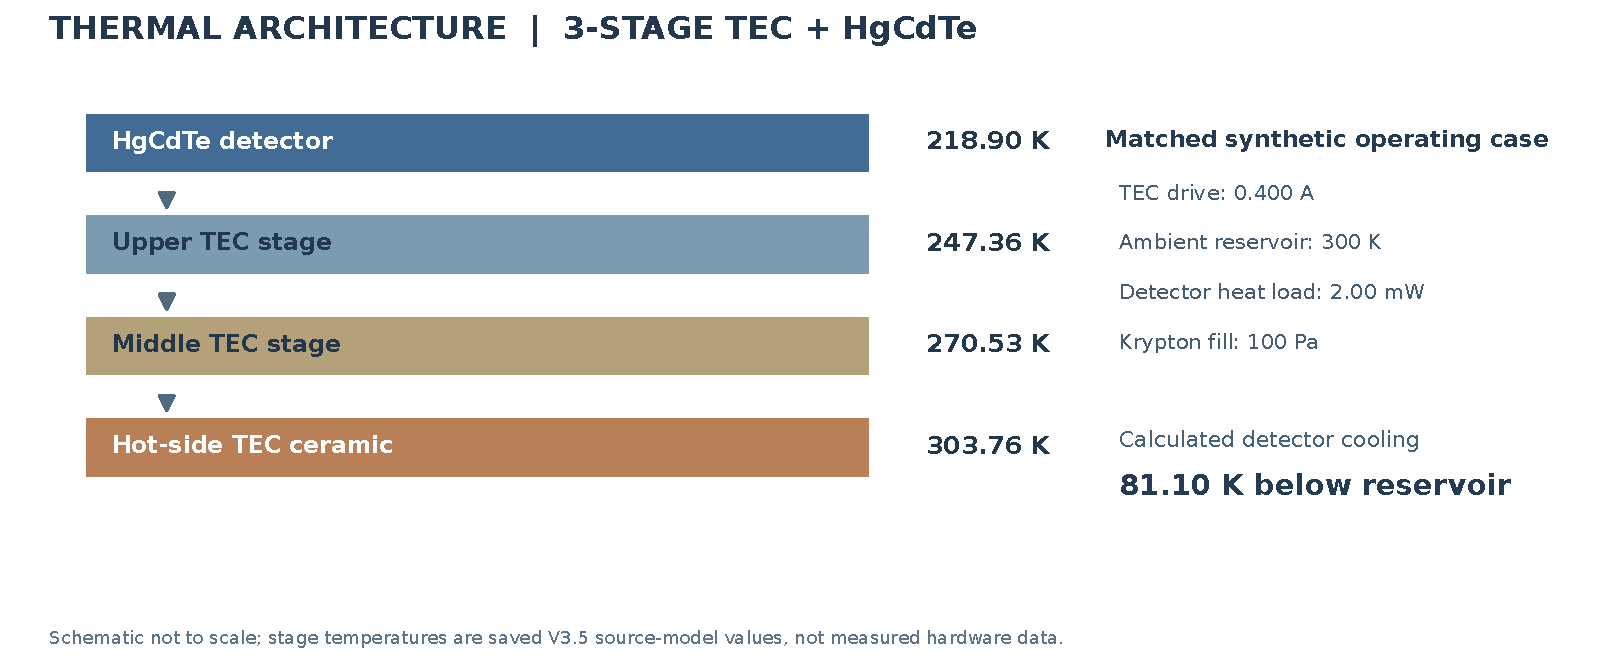
\includegraphics[width=.97\linewidth]{figures/cover_thermal_architecture.pdf}\end{center}
\vspace{3mm}
{\small Conceptual thermal architecture of the current V3.5 operating point, with calculated hot-side ceramic and detector temperatures. This is a source-data schematic, not a geometrically scaled rendering or measured device. The true formed-foil CAD is shown later in the cooler-layout section.}
\vfill
{\color{navy}\rule{\linewidth}{1pt}}
{\small\textbf{Evidence standard.} Calculated performance, material-property assumptions, source dimensions, and unresolved physical losses are separated throughout. A low residual demonstrates energy accounting, not measured detector performance.}
\clearpage
\section*{Engineering summary}\addcontentsline{toc}{section}{Engineering summary}
\textbf{Question.} How cold can a compact, three-stage thermoelectric cooler hold an HgCdTe photoconductor when heat must leave through a real package, and what thermal or electrical losses most threaten its performance?

A synthetic cooler is examined with four alumina substrates, 44 P/N thermoelectric couples divided among three stages (29 hot-side, 11 middle, 4 cold-side), soldered contacts, patterned metallization, supported formed copper-foil electrical transitions, and a HgCdTe die mounted at the cold end. The device occupies a proposed nine-pin metal package with a window. The interior is \emph{physically designed}, but its material grades and joint specifications are not measurements of a commercial cooler.

\textbf{Nominal operating condition:} 0.400 A applied TEC current; 300 K ambient thermal reservoir; 2.00 mW imposed detector heat; 100 Pa krypton in the enclosure; literature-derived P/N transport curves and selected contact/heat-sink parameters. The calculated operating point is
\[
\boxed{T_{\mathrm{detector}}=218.900\ \mathrm{K}}\qquad
\boxed{V_{\mathrm{TEC}}=1.489\ \mathrm{V}}\qquad
\boxed{P_{\mathrm{electrical}}=0.596\ \mathrm{W}}.
\]
This corresponds to an \emph{approximately 81.10 K detector-to-reservoir temperature difference}, not a validated maximum TEC temperature drop or measured commercial specification. V3.3 without the formed copper bridge gave 210.625 K, while V3.4 with interstage copper and a combined power-lead approximation gave 218.833 K. The current V3.5 model resolves both TEC supply leads on their actual ceramic contact faces and produces 218.900 K, a total \textbf{8.275 K} above V3.3 under the declared reference hypotheses. The original V3.3 cavity-off/on comparison remains useful but is a separate earlier model-generation experiment.

\textbf{Most important physical qualification:} The newer electrical design removes the long unsupported copper-bar arrangement in favor of short formed foil links and a three-foot return, with defined ceramic landing pads. The current thermal calculation includes individually modeled P/N legs, 3D heat spreading through the four ceramics, solder/contact \emph{electrical} losses, and effective package heat exchange. V3.5 retains the actual formed copper bridges and their three-foot return as an energy-conserving \emph{reduced} electrical/thermal network, and corrects the two package-pin supply wires to original ceramic face 8 and 36. Its nominal Cu-lead temperature is 218.900 K. The nickel-like lead hypothesis differs by only +0.015 K, while a deliberately severe Cu interstage thermal-interface resistance changes the nominal result by \textbf{-6.276 K}. The extreme contact case is a sensitivity, not a recommended solder design. True 3D metal current crowding, solder thermopower and measured material/contact properties remain unqualified. Neither the former 210 K result nor the new 219 K result constitutes hardware validation.

\textbf{Engineering use:} The calculation identifies where energy is pumped, dissipated, parasitically imported or rejected, including about 110.6 mW removed from the hotter substrate through the V3.5 formed copper interstage connections, of which 87.2 mW enters the upper substrate; it predicts temperature, voltage and stage-by-stage heat loads under declared assumptions; and it provides a reusable starting point for evaluating metallurgy, foil geometry, contact thermal resistance, gas pressure and heat-sink design. Numerical mesh details and document-history evidence appear \emph{after} the physical assessment.
\clearpage
\vspace{2mm}\par\textbf{Expanded TEC/TO design studies (9 November 2026).} New separately audited source-architecture results examine matched P/N material transport screens, finite TO mounting resistance and matched-temperature TEC power, high-temperature transport-law continuation, and eight cavity gas/pressure and current cases. At 0.400 A and 30 kPa, the predicted top ceramic is 218.845 K with Kr, 219.277 K with Ar and 219.703 K with nitrogen; these values use a declared effective 3 mm gap, not a native three-dimensional cavity solution. The original geometric, electrical, temperature-field and numerical appendices are retained.\par
\begingroup\small\setlength{\parskip}{0pt}\tableofcontents\endgroup\clearpage

\noindent\textbf{Reader navigation.} The main assessment follows the physical device: construction and governing transport, interconnects and TO thermal paths, accepted operating conditions and sensitivity studies, then historical baseline comparisons, numerical verification and reproduction details. Historic simulations are retained as distinct source-model generations; the latest contact and material studies have explicit qualification limits.\par\medskip
\section{Device construction and thermal architecture}
Four nominal ceramic plates have square footprints 6.4, 5.2, 3.8 and 2.4 mm, each 0.5 mm thick. Eighty-eight P/N legs are 0.4 by 0.4 by 0.5 mm each, grouped into 58, 22 and 8 legs from hot to cold. The TEC supply is connected to header pins 1 and 9; the HgCdTe photoconductor has separate bias contacts on pins 7 and 8. The gold-colored contact patterns on the ceramic are internal series metallization and solder lands, \emph{not} the external positive and negative power terminals. The exported reference contains 824 CAD solids and 176 solder joints, 89 insulated TEC electrical nets, and formed internal metal links.
\fig[.88]{cad_package_shaded}{png}{Physical arrangement of the proposed packaged HgCdTe device. Left: closed metal cap and optical window above the nine-pin header. Right: identical source-derived assembly with cover removed, exposing the thermoelectric stack, foil connections, TEC supply leads, and separate detector wiring. The external lead tails below the header are cropped for clarity; the mechanical assembly is synthetic, not a manufactured module.}
The original long, unsupported copper routing was rejected. The replacement has formed Cu-family foil tabs across nets 58 and 80, plus an extended three-foot return net 88 with a real middle thermal landing. Its design uses patterned ceramic metallization and finite solder footprints. The selected foil section is 0.300 by 0.030 mm; its bend radius is 0.075 mm; finished foot joints are specified at 20 plus/minus 5 micrometres. No measured current rating or fatigue qualification follows.
\fig[.88]{cad_package_pinout}{pdf}{Source-registered physical top-projection of all nine header feedthrough centers in millimetres. Blue pins 1 and 9 connect the thermoelectric series path; orange pins 7 and 8 connect the separate HgCdTe photoconductor circuit. The pin-location guide is not the real machined header outline. No unverified polarity or wire-harness assignment is implied.}

\section{Cooler layout and supported interstage connections}
The shaded views below tessellate the original 824-body source geometry using a true per-pixel depth buffer. The previous mean-face-depth renderer wrongly displayed hidden metallization through ceramic solids. This rendering is neither a reconstructed cooler nor an exploded assembly. All plates, P/N legs and analytically bent copper foil links retain the source positions, widths, heights, polarities and original path radii. Compared with the wireframe, the opaque solid bodies make the differences from the rejected long copper-post construction readily visible.

\fig[.98]{tec_solid_inspection}{png}{Correctly depth-occluded replacement geometry from two orthographic views: four ceramic stages, 58/22/8 P/N legs, visible exposed metallization only, and actual formed copper-foil connections. The external case, leads and very thin buried film layers are intentionally omitted. Original analytic foil-bend paths are sampled for shaded display, without relocating any CAD features.}
\subsection{Actual interstage foil cross-sections}
The design uses two short supported formed copper-foil stage links (nets 58 and 80), and a longer stepped return (net 88). The last has two vertical steps and three physical feet, including an intermediate thermal landing. Unlike a generic connecting rod, its cross-section has nominal width 0.300 mm, thickness 0.030 mm and bend radius 0.075 mm. The foil is represented at actual thickness, not enlarged for visibility.

\fig[.98]{tec_formed_tab_sections}{png}{Y--Z sections reconstructed from the source analytic straight and circular-arc geometry at original coordinates, without exploded offsets. Pale blue regions indicate where ceramic cross-sections intersect each foil plane. The 30-micrometre copper thickness is drawn at true scale.}
This original-CAD visualization establishes the mechanical design, rather than a simulated copper current or temperature field. V3.4 and V3.5 now account for foil conduction, Joule loss and finite metal/ceramic thermal contacts with a conservative reduced multiport. True three-dimensional current crowding, metallization-sheet spreading, measured joints and actual fabrication remain outside the qualified model.
\section{Thermoelectric material behavior and heat pumping}
Each of the 88 axial P/N legs uses a signed 0.4 A series current and 32 longitudinal intervals. With \(z\) directed hot-to-cold, \(S(T)\) Seebeck coefficient, \(\rho(T)\) resistivity, \(k(T)\) conductivity, and signed current density \(J\), the constitutive conservation model is
\[
q=S(T)TJ-k(T){dT\over dz},\qquad
{dq\over dz}=J\left[\rho(T)J+S(T){dT\over dz}\right],\qquad
{dV\over dz}=\rho(T)J+S(T){dT\over dz}.
\]
Midpoint constitutive evaluation and damped Newton iterations enforce thermal and electrical conservation at local temperatures, including the boundary identity \(Q_h-Q_c=IV_{\mathrm{leg}}\). The material source is a 14-knot figure digitization of research P-HE and N-HE-1 specimens over 40--300 K. Above 300 K the code uses an \emph{unmeasured} one-quarter final-segment slope continuation; this is not a production material characterization.
\fig[.92]{v33_transport}{pdf}{Source-derived P/N research analog properties. The shaded/dashed extension beyond 300 K is explicitly assumed; 58 hot-stage leg contacts exceed the research marker range.}

\section{Heat spreading through ceramic substrates}
Each ceramic independently solves
\[
-\nabla\cdot(k_c\nabla T)=0,\qquad
K_{ab}=\sum_e\int_{\Omega_e}k_c\nabla N_a\cdot\nabla N_b\,d\Omega,\quad
b_a=\sum_f\int_{A_f}N_a q_f\,dA,
\]
with \(k_c=30\,\mathrm{W/(m\,K)}\) a selected constant-property alumina analogue. Original face-specific P/N leg heat and assumed joint/cavity contributions are distributed over native TRI3 pad faces; source-local pad means feed back into leg end temperatures. Four archived source meshes contain 4,936 / 4,085 / 1,986 / 784 TET4 elements, totaling 11,791 tetrahedra.
\subsection{Preserved spatial evidence: original V3.3 and current V3.5}
The original source-ceramic temperature field from the earlier V3.3 reference is retained below as a \emph{historical baseline}. Its thermal state omits the later copper-interstage multiport and independently located TEC lead boundary conditions; it must not be mistaken for a field from the present operating-point calculation.
\fig[.96]{v33_ceramic_fields}{pdf}{Preserved original V3.3 four-ceramic spatial FEM fields and source tetrahedral surface triangulations, calculated for the older reference without the V3.4 formed-copper heat network or V3.5 corrected TEC lead-pad heat. This is the original evidence, not a replacement or a claim of validated device temperature.}
\clearpage
\subsection{Current V3.5 source-ceramic temperature field}
The revised V3.5 temperature plots use the \emph{same original ceramic discretization} but a different, more complete interstage copper/terminal-wire heat budget. These two figures intentionally coexist: the old field is preserved, and the updated field is appended with its own physical assumptions.
\fig[.96]{v35_original_spatial_ceramic_fields}{pdf}{Accepted current V3.5 operating-point temperature on the original frozen 11,791 source-ceramic TET4 elements. The original upper-surface TRI3 boundary is colored by the saved spatial FEM nodal solution at 0.400 A, 300 K, 2 mW detector load, 100 Pa krypton and nominal Cu contacts. These are actual solved ceramic temperature fields; there is no claim of full 430-domain bulk-metal electrothermal FEM.}
The four fields share their temperature gauge and stage heat exchange with the nonlocal reduced network. This is a single-mesh spatial result; no independent mesh-converged thermal accuracy bound is available.
\clearpage
\section{Electrical routing and interstage heat leakage}
The CAD conductor graph verifies all 88 legs as articulation vertices in the pin-1-to-pin-9 series circuit: removing any one leg disconnects the two terminals. Native transitions pass from P leg 57 to N leg 58 through tab 58, and from P79 to N80 through tab 80. The final leg P87 is connected to pin 9 through stepped return 88. These checks prove intended topology but not the temperature-dependent electrical or thermal properties of the connections.
\fig[.92]{v33_topology_legible}{pdf}{Actual saved stage-specific P/N leg centroids and plate footprints. This verifies the source positions used in the working hybrid; it does not depict a solved copper-tab thermal field.}
For a uniform slender conductor with temperature-dependent material properties,
\[
 R_e=\int_0^L{\rho(T,s)\over A(s)}\,ds,\qquad
 G_{\rm th}=\left[\int_0^L{ds\over k(T,s)A(s)}\right]^{-1},\quad
 P_J=I^2 R_e.
\]
The registered neutral path lengths are 1.96062 mm (net58), 1.97062 mm (net80), and 3.70624 mm (return88). Using a uniform 0.300 by 0.030 mm section, illustrative \(\rho_{\rm Cu}=1/(58\times10^6)\,\Omega{\rm m}\) and \(k_{\rm Cu}=385\,\mathrm{W/(m\,K)}\) yields the approximate geometry-only screen below.
\fig[.92]{tab_screen}{pdf}{Historical pre-V3.4 screening of idealized uniform-bar electrical and thermal copper coefficients. Actual formed-tab bends, patterned multilayer film, contact drops, variable temperatures, Joule partition and intermediate return landing are not resolved. The return is not correctly represented by a single two-terminal thermal conductance.}
The competing design goals are explicit: reducing electrical resistance through a larger cross-section increases passive thermal coupling. This geometry-only conductance screen is archived from the pre-V3.4 design assessment; the source-face, three-terminal return multiport is now included in V3.4/V3.5 and documented earlier. Its assumed interface and bulk properties, rather than the electrical path topology, now dominate outstanding thermal uncertainty.

\section{Electrical contacts, solder joints and dissipative heating}
The preserved source-solder model assumes 176 solder bodies of 35 micrometres thickness and 0.16 mm$^2$ area, with assumed SnSb resistivity \(1.7\times10^{-7}\ \Omega\,{\rm m}\) and 352 assumed metal-interface specific resistances \(r_c^{\prime\prime}=10^{-11}\ \Omega\,{\rm m}^2\). For each joint the resistance is
\[
R_j=\rho_{\rm SnSb}{L_j\over A_j}+2{r_c^{\prime\prime}\over A_j},\quad
R_{\rm all}=0.028545\ \Omega,\quad I^2R_{\rm all}=4.56720\ {\rm mW}.
\]
The implementation places 25.950 micowatts per source joint into its neighboring ceramic pad. This assumes the entire joint Joule heat reaches a ceramic and omits finite thermal-contact drops, interfacial thermopower and nonlocal copper-network heating. The four ceramic applied-joint terms, in mW, are [1.50510, 2.07600, 0.77850, 0.20760].
External TEC supply Cu wires and detector Au bonds are separate electrical/thermal links. \emph{The formed tabs/return are accounted for by the separate V3.4/V3.5 reduced copper network described earlier, not by the solder-only term above.}

\section{Package parasitic heat loads and thermal rejection}
The reference forward case imposes a 300 K cap/window/ambient thermal reservoir, a 100 Pa krypton environment, an effective 3.0 mm gas gap, accommodation 0.8, and nominal gas conductivity knots \(k_{\rm Kr}(200,300,400\,{\rm K})=(0.0064,0.0095,0.0122)\ {\rm W/(m\,K)}\).
Gray radiation uses assumed emissivities \(\epsilon_{\rm cap}=0.20\), \(\epsilon_{\rm ceramic}=0.80\), and \(\epsilon_{\rm window}=0.10\), with selected effective view factors. The source effective exposed surface areas are [12.60, 8.68, 4.76, 1.00] mm$^2$. The generic exchange terms are
\[
Q_{{\rm gas},i}=G_{\rm eff,i}(p,T)(T_\infty-T_i),\qquad
Q_{{\rm rad},i}=\epsilon_{{\rm eff},i}\sigma A_iF_i(T_\infty^4-T_i^4).
\]
These are \emph{effective engineering closures}, not cavity fluid dynamics, true free-molecular transport, exact exposed-face loads, spectral window modeling or full radiosity.
\fig[.92]{v33_cavity_loads}{pdf}{Archived V3.3 cavity contributions: total gas 3.892553 mW, gray radiation 0.624076 mW, combined heat into cold components 4.516629 mW. The reservoir carries an equal and opposite signed load.}
\begin{center}\small\begin{tabular}{lrrr}\toprule
Cold destination & Kr gas (mW) & Gray rad. (mW) & Total (mW)\\\midrule
\cavityrows
\bottomrule\end{tabular}\end{center}
An effective header/TIM/radiator resistance of approximately 4.8334 K/W carries heat to the warm sink. Neither mount pressure nor material lot is an experimental datum. The cavity load is redistributed to native \emph{upper metal-pad} sources in the current model; thermal gradients on exposed bare ceramic faces are not thereby demonstrated.

\section{Terminal wires, soldered TO pins, and thermal uncertainty}
The TEC power supply must reach the miniature cooler through real wires soldered to the metal-package feedthrough pins. As supplied, these wires may be substantially longer than the \emph{installed} length and are cut to fit the TO header. Only the final internal conductor from the cooler landing to each package pin contributes to the source ceramic-to-pin heat and current path; factory surplus outside the completed joint does not add thermal length to that connection.

The current source-derived layout has two independent, 0.200 mm diameter power leads. Pin 1 is connected to original ceramic face \textbf{8} over a 3.451 mm route; pin 9 is connected to original ceramic face \textbf{36} over a 4.965 mm route. The V3.4 average-hot-temperature model incorrectly combined both heat loads onto face 36. In the original saved ceramic field the two landings were near 303.94 and 298.39 K, respectively; they therefore need not exchange heat in the same direction with the 300 K header.

At \emph{matched} 0.400 A, 300 K external reservoir, 2 mW detector heat and 100 Pa krypton, the improved three-stage calculations give:
\begin{center}\small
\begin{tabular}{lrrr}\toprule
Selected physical hypothesis & Detector (K) & TEC V & Input (mW)\\\midrule
\vfiveoperatingrows
\bottomrule\end{tabular}
\end{center}
The source-corrected copper-wire model predicts \textbf{218.900 K}, 0.067 K above the original V3.4 218.833 K. A same-geometry pure-nickel-like assumption raises that value by \textbf{0.015 K}. In contrast, raising the \emph{interstage formed-copper joint} thermal-interface areal resistance from \(10^{-6}\) to an extreme \(10^{-4}\ {\rm m^2 K/W}\) lowers calculated die temperature to \textbf{212.624 K}. This is a deliberately severe interface hypothesis, not measured solder behavior or an endorsement of unreliable joints.
\fig[.95]{v35_full_system_scenario_temperature}{pdf}{Two explicitly different horizontal scales for accepted full-system simulations at the same 0.400 A, 300 K, 2 mW and 100 Pa condition. Left: 6.276 K sensitivity to an extreme Cu interstage thermal-contact hypothesis. Right: millikelvin departures associated with the corrected terminal-lead model and selected Cu/Ni-like material properties. These are hypothetical design sensitivities, not measured uncertainty intervals.}
\clearpage
\subsection{Separate source contact heat, lead material, and cut length}
For lead \(i\) with source internal length \(L_i\), radius \(r_i\), electrical resistivity \(\rho_i\) and thermal conductivity \(k_i\), use
\[
 A_i=\pi r_i^2,\quad R_i=\rho_i L_i/A_i,\quad
 G_i=k_i A_i/L_i,\quad
 Q_{i\to c}=G_i(T_{\rm pin}-T_{c,i})+\tfrac12 I^2 R_i.
\]
The one-half lead Joule partition is a reduced axial model assumption; the remaining half is rejected at the external pin. All terminal electrical \(I^2R\) enters the TEC voltage/power balance, without double counting the externally rejected half as cold-side heat.

\begin{center}\small
\begin{tabular}{lrrr}\toprule
Fully solved wire case & Pin 1 heat (mW) & Pin 9 heat (mW) & Wire Joule (mW)\\\midrule
\vfiveleadrows
\bottomrule\end{tabular}
\end{center}
Signed heat is positive \emph{into} the ceramic. With 300 K pin temperatures, pin 1 removes heat from its warmer ceramic while pin 9 imports heat to a cooler landing. Thus calculating both leads from one average hot-side temperature loses genuine local heat-flow information.

Nominal copper properties are \(k=400\ {\rm W/(m\,K)}\), \(\rho=1.72\times10^{-8}\ \Omega{\rm m}\); the illustrative nickel-like case uses \(k=90\ {\rm W/(m\,K)}\), \(\rho=7.00\times10^{-8}\ \Omega{\rm m}\). Actual manufacturer supplies should not be identified by color or visual impression: TEC Microsystems and RMT specify \emph{tinned copper} as default, with manufacturer-dependent terminal options. The FeCrAl/Kanthal-like resistance-wire case is included only as a fixed-field counterfactual: at 0.400 A and the same 0.200 mm diameter geometry, its assumed resistance is 0.3884 \(\Omega\), generating \emph{62.15 mW} of electrical heat. No such lead alloy has been identified on this physical cooler.
\fig[.95]{v35_fixed_field_lead_heat_screen_legible}{pdf}{Lead material comparison at one frozen real V3.4 3D ceramic temperature field. Unlike the operating-point table above, this diagnostic is a fixed-field thermal/electrical source screen, not a nonlinear detector-temperature prediction.}
\clearpage
\subsection{The larger uncertainty: interstage copper and ceramic joint conductance}
The three formed stage bridges carry both electrical current and parasitic heat. At each source-defined foil foot of area \(A_c=0.060\ {\rm mm^2}\), the provisional thermal contact conductance is \(G_c=A_c/r_{T,c}''\). The nominal \(r_{T,c}''=10^{-6}\ {\rm m^2 K/W}\) is a selected non-measured contact assumption. A higher areal resistance reduces the conductive bypass in this model, but may be impractical or conflict with electrical continuity, solder fatigue, and actual fabrication.

Holding the \emph{original} V3.4 source pad temperatures fixed, the first-pass upper-ceramic copper heat is:
\begin{center}\small
\begin{tabular}{rr}\toprule
Assumed \(r_{T,c}''\) (m$^2$ K/W) & Upper-plate Cu heat (mW)\\\midrule
\vfivecontactrows
\bottomrule\end{tabular}
\end{center}
\fig[.90]{v35_fixed_field_interstage_contact_screen_legible}{pdf}{Source-pad-fixed heat-flux response to copper-foil interface assumptions. These intermediate screening fluxes are deliberately distinct from the three accepted fully coupled V3.5 operating-point results.}
In the full-device copper-reference calculation, the upper plate receives \textbf{87.173 mW} through the Cu network and its hot stage-3 boundary is \textbf{247.359 K}. Under the severe interface hypothesis, those values become \textbf{21.697 mW} and \textbf{238.856 K}; the detector then equilibrates to 212.624 K. An 0.015 K lead-material change versus a 6.276 K copper-joint sensitivity identifies the next physically important question: \emph{what is the realistic electrical and thermal interface law for the formed Cu foil, its solder feet, and the plated ceramic?}
\subsection{Independent verification, limitations, and model use}
Each V3.5 case uses the original 88 nonlinear axial P/N legs and four spatial ceramic FEMs with native source face heat. Three matched reference conditions converged with the following independent checks:
\begin{center}\scriptsize
\begin{tabular}{lrrr}\toprule
Scenario & Max pad update (K) & Stage residual (W) & Global residual (W)\\\midrule
\vfivecheckrows
\bottomrule\end{tabular}
\end{center}
The stricter requirements remain below \(3\times10^{-7}\) K for the spatial update and \(10^{-8}\) W for independently reconstructed stage and global energy balances. A separate audit re-evaluates both wire conductances/resistances from the unmodified source CAD, all three Cu bridge metal/contact networks (including the third thermal return port), all stage energy budgets and terminal voltage. The documentation and plots consume only frozen accepted results; no new PDE solve is performed during report generation.

The wire and Cu laws are declared approximations, not measured low-temperature transport, OEM process tolerances or an as-manufactured TO feedthrough temperature solution. Neither the 0.200 mm diameter nor the installed route exactly identifies a vendor assembly. The next physical priority is credible solder/joint thermal resistance, plated-film heat spreading and conductor temperature-dependent properties. Cut-to-size factory terminal leads should be assigned the \emph{installed} ceramic-to-pin length; an off-device surplus must never be treated as extra insulation that improves TEC temperature.


\section{Original V3.4 copper-bridge result and its physical explanation}
A thermoelectric cooler transfers heat toward its hot side while electrical interconnects must also cross between ceramic stages. The three short formed copper-foil connections in the current cooler provide a real electrical path, but they simultaneously create passive conductive paths that partially undo the cooling. This effect is absent from the original V3.3 prediction. A new V3.4 calculation adds the actual two-foot and three-foot link topology with physically separate ceramic-pad thermal terminals.

At the \emph{same} 0.400 A input, 300 K heat reservoir, 2.00 mW detector heat and 100 Pa krypton setting:
\begin{center}\small
\begin{tabular}{lrrr}\toprule
Calculated quantity & V3.3 & V3.4 with copper & Change\\\midrule
\vfourmetricrows
\bottomrule\end{tabular}
\end{center}
Although the predicted electrical power falls, the detector is \textbf{8.208 K warmer}. The important loss mechanism is \emph{parasitic stage-to-stage conduction} through the copper, not simply additional resistive power dissipated in the tabs.
\fig[.95]{v34_copper_stage_temperature_comparison}{pdf}{Solved source-ceramic stage and detector temperatures in V3.3 versus V3.4 at matched source assumptions. V3.4 adds a geometry-derived, finite-contact copper heat network; this is a conditional theoretical comparison, not measured or full 3D copper-metal fields.}
\clearpage
\subsection{Copper heat paths and their thermal consequences}
The original CAD includes copper-foil tabs across electrical nets 58 and 80 and a stepped return at net 88. Their original contact sites on the three source ceramic planes are:
\[
{\rm net58}:\ 38\to75,\qquad
{\rm net80}:\ 79\to105,\qquad
{\rm net88}:\ 36\to74\to104.
\]
The actual bridge foil width/thickness are 0.300/0.030 mm. Heat transfer uses the actual \emph{center-to-center} solder-foot spans, not the full unsupported length of each tab. Net88 has an intermediate supported landing and therefore three separate thermal terminals. The model does not treat that landing as insulated.

For a foil segment \(i,j\) and finite contact \(c,i\):
\[
G_{ij}=k_{\rm Cu}A/L_{ij},\qquad
R_{ij}=\rho_{\rm Cu}(T_{ij})L_{ij}/A,\qquad
G_{c,i}=A_{c,i}/r_{T,c}'',
\]
where the provisional material laws use \(k_{\rm Cu}=385\ \mathrm{W/(m\,K)}\),
\(\rho_{\rm Cu}(T)=1.724\times10^{-8}[1+0.0039(T-293.15)]\ \Omega\,{\rm m}\),
\(r_{T,c}''=10^{-6}\ \mathrm{m^2K/W}\), and \(r_{e,c}''=10^{-11}\ \Omega\,{\rm m^2}\). These are \textbf{selected engineering hypotheses}, not identified foil or solder-lot properties.

The node equation
\[
\sum_j G_{ij}(T_i^{\rm foil}-T_j^{\rm foil})
+G_{c,i}(T_i^{\rm foil}-T_i^{\rm ceramic})
=P_{J,i}
\]
sends local conduction and Joule heat to the original 3D ceramic-pad faces. The signed results below are reported as \emph{heat into ceramic}; negative values indicate the foil removes heat:
\begin{center}\small
\begin{tabular}{lrrrr}\toprule
Foil connection & Hot (mW) & Mid (mW) & Upper (mW) & Joule (mW)\\\midrule
\vfourcopperrows
\bottomrule\end{tabular}
\end{center}
The copper network removes approximately 108.5 mW from the hot ceramic while depositing 87.0 mW in the upper ceramic. These are \emph{redistributed} heat flows, not net external heat creation. Their stage total equals the copper circuit's 2.080 mW of electrical Joule dissipation.
\fig[.95]{v34_copper_face_heat_budget}{pdf}{Original-CAD-face copper heat flows from accepted V3.4: individual networks at nets 58, 80 and 88. Positive denotes heat entering ceramic. Net88's middle contact has its own nonzero heat flux.}
\clearpage
\subsection{Resulting three-stage heat pumping and numerical checks}
\begin{center}\small
\begin{tabular}{rrrrr}\toprule
TEC stage & Number of legs & \(Q_c\) (mW) & \(Q_h\) (mW) & Voltage (V)\\\midrule
\vfourstagerows
\bottomrule\end{tabular}
\end{center}
The upper-stage hot boundary increases from 236.16 K (V3.3) to 247.27 K (V3.4). The stage therefore operates across a materially altered thermal environment while still providing approximately 4.910 mW of cold-side heat pumping.

Two earlier fixed-point attempts remain archived as \textbf{STOP}; the second passed a coarse pad-temperature threshold but failed the final energy test. The accepted third attempt meets the tighter 3\(\times10^{-7}\) K temperature-update criterion after \textbf{19} outer steps, without changing the source physics:
\begin{center}\small
\begin{tabular}{lr}\toprule
Independent engineering check & Absolute residual\\\midrule
\vfourcheckrows
\bottomrule\end{tabular}
\end{center}
A separately implemented read-only audit reconstructs copper Joule, all three stage heat balances and the hot-reservoir balance from the saved original-face and node data, without rerunning the coupled PDE. The 3D FEM still solves \emph{only the ceramics}; the copper model remains a source-connected 1D heat/electric network with assumed contacts. These residuals establish internal conservation, not an experimental uncertainty interval. The principal next uncertainty is whether actual copper conductivity, foil/joint resistance, plated sheet spreading and geometry tolerances preserve the calculated 8.2 K shift.

\section{Current versus cooling performance: an operating envelope (V3.6)}
The previous V3.5 model demonstrated a realistic source-connected 0.400~A operating point, but a hardware engineer needs to know how detector temperature and dissipated electrical power change with \emph{TEC drive current}. V3.6 varies only the imposed current and detector heat load, using the \emph{same} 88 source P/N transport legs, 11,791 ceramic tetrahedra, copper-foil interstage links, actual terminal feedthrough connections, krypton cavity and mounting sink assumptions. No material law or geometry was fitted to produce this curve.

At 300~K mounting reservoir, 2.00~mW detector heat and 100~Pa krypton, four independently conserved operating points give:
\begin{center}\small
\begin{tabular}{rrrr}\toprule
TEC current (A) & HgCdTe T (K) & Terminal V (V) & Input (W)\\\midrule
\vsixcurrentrows
\bottomrule\end{tabular}
\end{center}
\fig[.97]{v36_current_temperature_power_legible}{pdf}{Four full-system source-model cases showing the decrease in detector temperature and increasing electrical input from 0.25 to 0.60~A. The line segments connect individually solved points; they are not a fitted continuous performance or safe-current curve. Other parameters are fixed at the nominal V3.5 physical hypotheses.}
The upper-stage hot substrate cools from 260.43~K at 0.25~A to 237.36~K at 0.60~A, while the mounting-side TEC ceramic warms from 301.66 to 307.71~K because it must reject more heat through finite package impedance. The extra electrical cost of a further kelvin of detector cooling rises markedly:
\begin{center}\small
\begin{tabular}{rrrr}\toprule
Current step (A) & Cooling gained (K) & Extra input (mW) & Incremental mW/K\\\midrule
\vsixcostrows
\bottomrule\end{tabular}
\end{center}
\par\nopagebreak[4] No minimum in detector temperature or safe current rating is claimed beyond the four tested conditions; increasing current still improved cooling at the upper tested 0.60~A boundary. The power budget is \emph{module terminal input}, not the entire external power-supply wall consumption.
\subsection{Sensitivity to real detector heating}
At fixed 0.400~A, an imposed thermal load is an essential proxy for absorbed photons, bias heating and parasitic package heat before the HgCdTe transport physics is self-consistently integrated. The following points resolve the full TEC--ceramic--package feedback, not a single isolated thermal resistance:
\begin{center}\small
\begin{tabular}{rrrr}\toprule
Detector load (mW) & HgCdTe T (K) & TEC V (V) & Input (W)\\\midrule
\vsixloadrows
\bottomrule\end{tabular}
\end{center}
\fig[.87]{v36_detector_heat_load_response}{pdf}{Source-based thermal load sweep at fixed 0.400~A, 300~K sink and 100~Pa krypton. The calculated full-device temperature changes by about 0.311~K per additional milliwatt across the tested 1--6~mW range. The HgCdTe resistance, signal and noise are not yet solved from semiconductor transport.}
From 1 to 2~mW the observed secant is 310.734~K/W; from 2 to 6~mW it is 311.184~K/W. This approximately \textbf{311~K/W effective device thermal sensitivity} applies to the specified module and drive condition, not a measured intrinsic die thermal resistance. It demonstrates what the platform can now predict about tolerable bias/optical heat and electrical cost \emph{before} an HgCdTe device-transport model supplies that heat self-consistently.

\textbf{Numerical evidence and limitations.} All six cases retain 88 nonlinear leg solutions, original four source ceramic fields and source-to-pin metal face heat accounting; separate no-solve audits recomputed each stage, copper, lead and global balance below \(2\times10^{-9}\)~W. The unmodified 0.400~A/2.00~mW V3.5 reference is reproduced exactly. Two failed off-reference initializations were preserved and corrected by keeping the frozen 0.4~A heat budget during the first \emph{warm start}; all physical equations and \(3\times10^{-7}\)~K pad-update gates remain unchanged. These curves remain conditional on selected copper/solder, thermoelectric and mounting properties; no photoconductive gain, infrared detectivity or detector noise is inferred. All original earlier V3.3--V3.5 scientific results follow as independent historical evidence.
\clearpage

% Expanded TEC/TO package studies. This file is inserted into the ORIGINAL
% report.tex source; none of the existing sections, figures or appendices
% are deleted or replaced. All numbers use independently accepted saved states.
% No simulator or detector-transport solve is invoked by typesetting.
\clearpage
\section{Thermoelectric transport sensitivity in the current cooler}
\label{sec:current-material-sensitivity}
An operating-temperature prediction depends critically on the actual paired
P- and N-type material transport functions. The present synthetic cooler uses
the full source-leg count, ceramic spatial fields, and metal heat paths, but
its research-specimen \(S(T)\), \(\rho(T)\), and \(k(T)\) curves are not a
measured or manufacturer-qualified TEC material pair. It would therefore be
premature to quote a narrow error bar on the absolute cold-stage temperature.

To quantify the leverage of these properties, a controlled source-geometry
study changed one common P/N property factor at a time, with the original
geometry, stage count, foil connections, mounting, gas, and electrical drive
held fixed. Each point is a full 88-leg, four-ceramic nonlinear solution,
\emph{not} a scaled temperature inferred from an isolated thermocouple.
The study applied \(I_{\rm TEC}=0.400\) A, a 300 K external reservoir, 100 Pa
krypton, and a conditional auxiliary detector load obtained from
\(0.866025^2/R_{\rm die}(T)\) plus 0.500 mW absorbed heat. The illustrative
\(R_{\rm die}(T)\) law in this study is \emph{not} used to infer actual detector
performance; the gas study later in this assessment retains a strictly fixed
2.000 mW imposed heat load. Consequently the two experiment families
must not be interpreted as identical detector-loading conditions.

\begin{center}\small
\begin{tabular}{lrrr}\toprule
P/N property hypothesis & Device mount (K) & Top ceramic (K) & TEC input (W)\\\midrule
All source factors 1.00 & 218.900 & 218.807 & 0.595668\\
Thermal conductivity \(\times0.80\) & 207.812 & 207.716 & 0.616656\\
Thermal conductivity \(\times1.20\) & 227.627 & 227.536 & 0.579393\\
Seebeck coefficient \(\times0.90\) & 225.833 & 225.741 & 0.562663\\
Seebeck coefficient \(\times1.10\) & 212.515 & 212.420 & 0.631764\\
Electrical resistivity \(\times0.80\) & 216.563 & 216.470 & 0.523689\\
Electrical resistivity \(\times1.20\) & 221.313 & 221.221 & 0.668943\\\bottomrule
\end{tabular}
\end{center}

Under the \emph{selected, unequal} factor intervals, the total device-mount
temperature endpoint spans are \(19.815\) K for \(k\), \(13.318\) K for
\(S\), and \(4.750\) K for \(\rho\), respectively. The ranking is an
engineering screening result, \textbf{not} a statistical sensitivity ranking:
the factor ranges are deliberately different, and independently modifying
only one material property can be physically incompatible with a real
thermoelectric grade.
\begin{center}
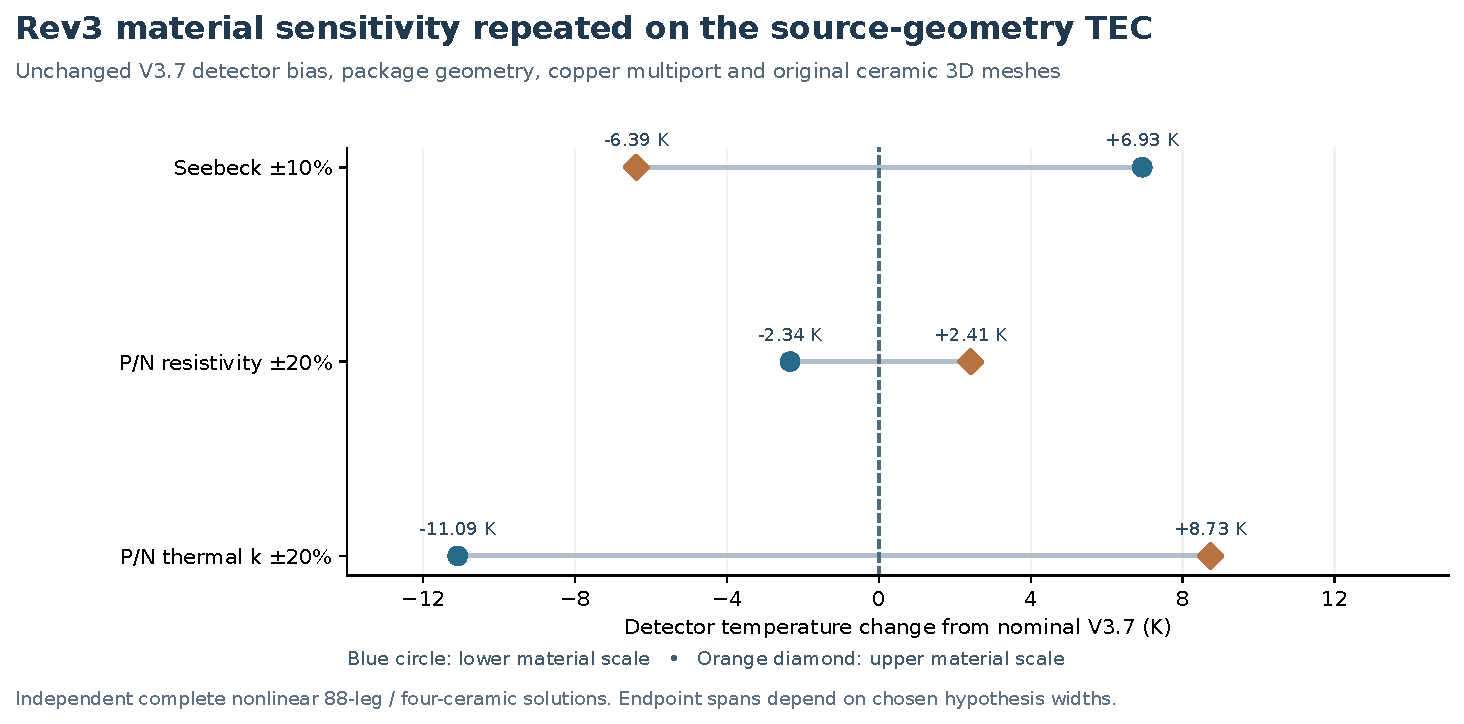
\includegraphics[width=.95\linewidth,height=.38\textheight,keepaspectratio]{figures/v38_source_material_response.pdf}
\par\vspace{1mm}{\small\textit{Figure \the\numexpr\value{figure}+1\relax.} Independently solved P/N
transport variations on the current full TEC/TO thermal architecture.
Source-property factor ranges are hypotheses, not production tolerances.}
\end{center}\stepcounter{figure}

\clearpage
\section{Package mounting and power required to hold a cold temperature}
\label{sec:mounting-and-matched-power}
Even with a fixed 300 K external reservoir, the hot ceramic is not
constrained to 300 K. Heat is rejected through an assumed finite package
mounting resistance. The nominal current reference uses
\(R_{\rm external}=4.833387\ {\rm K/W}\); the two controlled hypotheses add
5 or 10 K/W \emph{on top of} that reference. The combined
source-ceramic and 88-leg transport state was re-solved for each case, with
the same stated reference detector thermal-input law and TEC current.

\begin{center}\small
\begin{tabular}{rrrr}\toprule
Additional \(R_{\rm mount}\) & Total \(R_{\rm external}\) & Device mount \(T\) & TEC input\\
(K/W) & (K/W) & (K) & (W)\\\midrule
0 & 4.833387 & 218.900 & 0.595668\\
5 & 9.833387 & 220.393 & 0.604935\\
10 & 14.833387 & 221.856 & 0.613656\\\bottomrule
\end{tabular}
\end{center}
The fixed-current temperature penalties are \(+1.493\) K and
\(+2.956\) K for the added 5 and 10 K/W, respectively. Mounting resistance
is a package design variable and should not be confused with the cooler's
intrinsic material heat lift.

\begin{center}
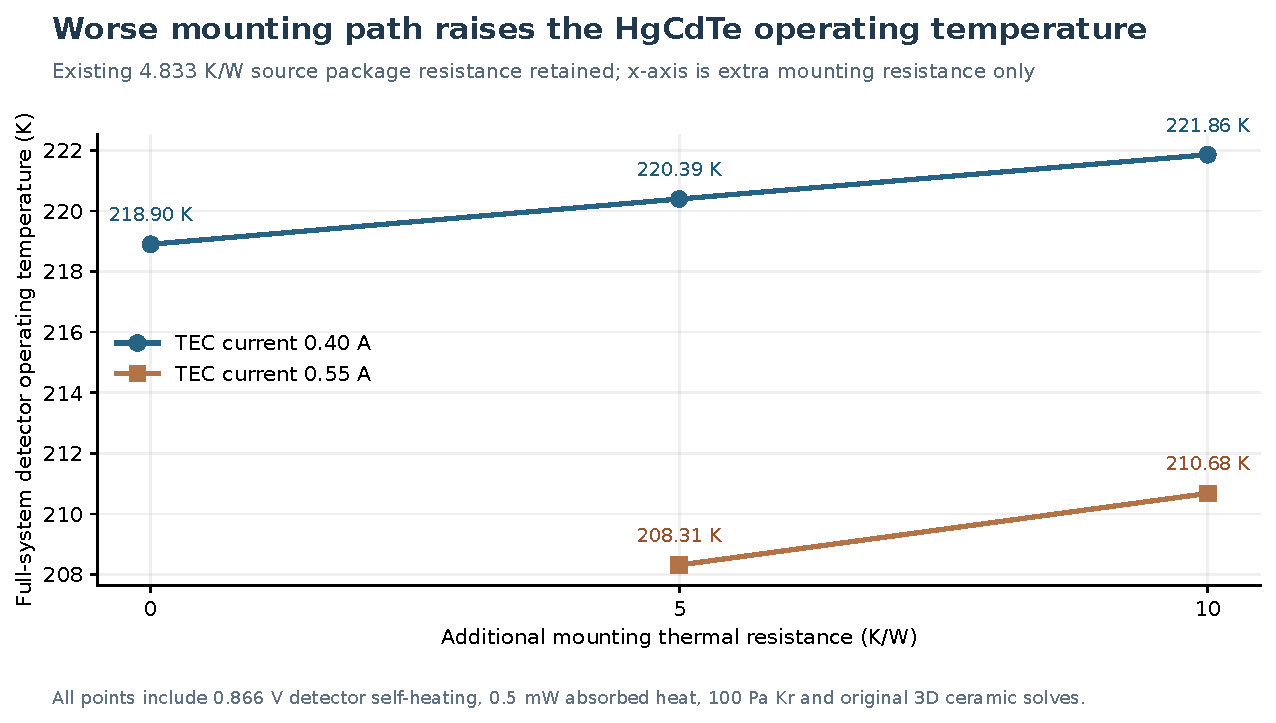
\includegraphics[width=.92\linewidth,height=.40\textheight,keepaspectratio]{figures/v38_package_sink_temperature.pdf}
\par\vspace{1mm}{\small\textit{Figure \the\numexpr\value{figure}+1\relax.}
The finite external mounting path changes the nonlinear whole-device
temperature distribution; the detector is not assigned a temperature rise
algebraically.}
\end{center}\stepcounter{figure}

A more practical procurement and instrument-design question is how
much additional electrical power is required to \emph{recover the same}
operating temperature when mounting quality deteriorates. Two new
registered, independently audited source solutions were obtained
after a bounded current bracket and one numerical correction.
These are \emph{actual} full-system solutions, not interpolated electric
power values.
\begin{center}\small
\begin{tabular}{rrrrr}\toprule
Extra \(R\) (K/W) & TEC \(I\) (A) & Device mount (K) & Input (W) & Power penalty\\\midrule
0 & 0.400000 & 218.900024 & 0.595668 & Reference\\
5 & 0.415286 & 218.892717 & 0.648375 & +8.85\%\\
10 & 0.433174 & 218.868845 & 0.712481 & +19.61\%\\\bottomrule
\end{tabular}
\end{center}
The maximum matched-temperature departure is just \(0.0312\) K.
The \(+10\) K/W mounting case demands approximately
\(116.8\) mW more \emph{TEC terminal power} to deliver essentially
the same device-platform temperature, under the chosen boundary
and material assumptions.

\clearpage
\begin{center}
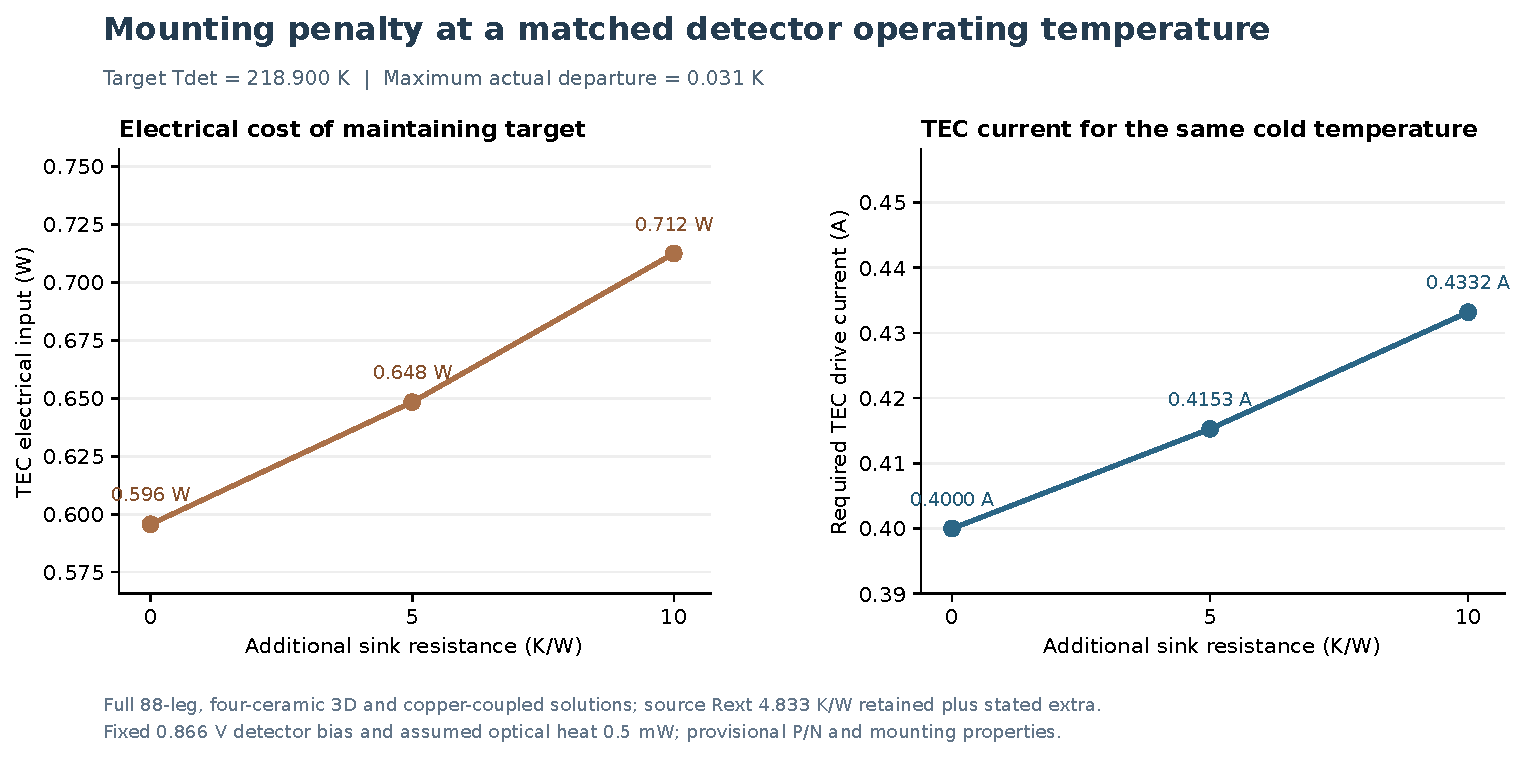
\includegraphics[width=.97\linewidth,height=.59\textheight,keepaspectratio]{figures/v38_matched_detector_temperature_power.pdf}
\par\vspace{2mm}{\small\textit{Figure \the\numexpr\value{figure}+1\relax.}
Calculated TEC current and terminal input required to maintain
near-equal mounting temperature as external resistance increases.
The comparison is not a measured OEM power rating or a global optimum.}
\end{center}\stepcounter{figure}

\subsection{Source-property validity above 300 K}
At the reference mounting condition the hot ceramic reaches about
303.8 K; with an additional 10 K/W it reaches about 309.5 K. The P/N
research curves have published markers through 300 K only. A separate
six-run continuation check held the original 40--300 K curves exactly fixed,
while assigning \(0\), \(25\), or \(100\%\) of the final source-curve
tangent beyond 300 K. Across those hypotheses the device temperature
spanned only \(0.0170\) K at nominal mounting and \(0.0782\) K under
the worsened mounting condition. The corresponding total TEC input-power
spans were \(0.545\) and \(3.115\) mW.

This result helps distinguish a \emph{particular extrapolation parameter}
from the much larger unqualified \emph{bulk P/N material grade} question.
It does not demonstrate that any of the three continuations is physically
correct, nor does it provide a statistical uncertainty interval.

\textbf{Engineering interpretation.}
Improving material-grade evidence and the mechanical/thermal TO mounting
interface should precede an expensive broad numerical sweep of speculative
high-temperature extrapolation functions. For any colder operating point,
state current, terminal voltage, heat load, source-temperature coverage,
mounting resistance, and the relevant electrical-power budget.

\clearpage
\section{Effect of cavity backfill on the TEC top stage}
\label{sec:package-backfill-current}
The packaged cooler is also subjected to a potentially substantial heat
leak from warm internal surfaces. A controlled eight-case study has now
re-solved the \emph{same} source-based TEC with rarefied-to-continuum
Kr, Ar and N$_2$ backfill conditions. To separate cavity transport from
detector-specific electronics, these simulations use a fixed
\(\boxed{Q_{\rm die}=2.000\ {\rm mW}}\) rather than an
electrical-resistance or optical absorption calculation.
The principal comparison holds
\(I_{\rm TEC}=0.400\ {\rm A}\) and external temperature 300 K.

\begin{center}\small
\begin{tabular}{lrrrr}\toprule
Backfill & Top ceramic & Device mount & Gas heat & TEC power\\
 & (K) & (K) & (mW) & (W)\\\midrule
Vacuum, gas off & 218.353 & 218.437 & 0.000 & 0.596111\\
Kr, 100 Pa & 218.807 & 218.900 & 3.420 & 0.595668\\
Kr, 30 kPa & 218.845 & 218.939 & 3.724 & 0.595630\\
Kr, 101.325 kPa & 218.845 & 218.939 & 3.725 & 0.595630\\
Ar, 30 kPa & 219.277 & 219.380 & 6.966 & 0.595209\\
N$_2$, 30 kPa & 219.703 & 219.815 & 10.170 & 0.594792\\
N$_2$, 101.325 kPa & 219.703 & 219.815 & 10.172 & 0.594792\\\bottomrule
\end{tabular}
\end{center}

At the same 30 kPa nominal pressure, nitrogen is \(0.8753\) K
warmer than krypton at the device mounting node and imports an
additional \(6.446\) mW of gas heat. Argon lies between the two.
Disabling gas conduction entirely gives a \(0.4634\) K cooler
mounting condition than 100 Pa Kr, while leaving solid and radiative
conduction active. No numerical result is assigned to a manufacturer
or a known production-gas recipe.

\begin{center}
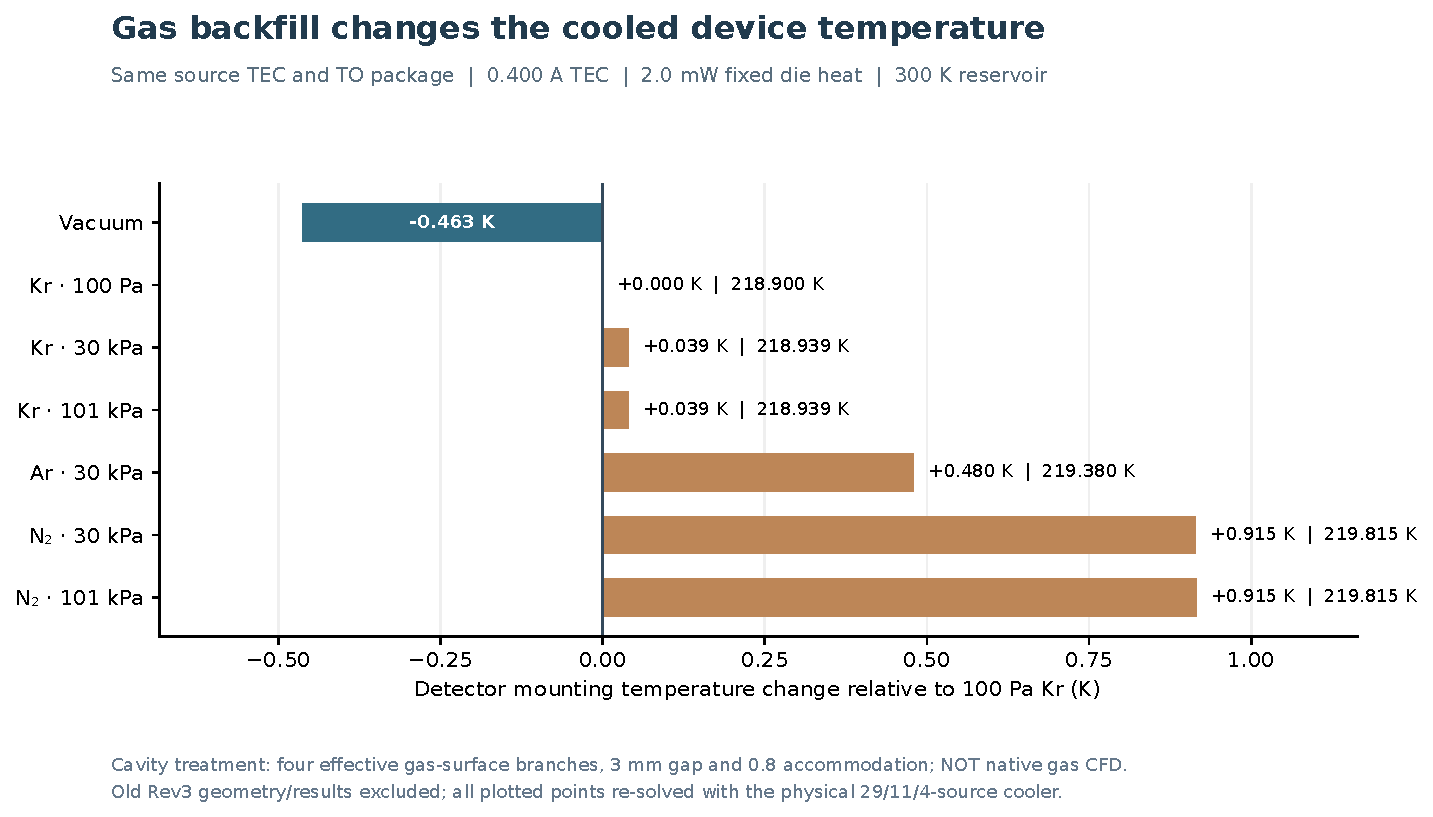
\includegraphics[width=.95\linewidth,height=.42\textheight,keepaspectratio]{figures/v311_backfill_species_pressure_cold_temperature.pdf}
\par\vspace{1mm}{\small\textit{Figure \the\numexpr\value{figure}+1\relax.}
Backfill gas and pressure sensitivity of the
device-side mounting temperature. The top TEC ceramic is a distinct
lower-temperature node; both are listed in the accompanying table.}
\end{center}\stepcounter{figure}

\clearpage
\section{Gas heat-transfer mechanism and its uncertainty}
\label{sec:gas-model-fidelity}
The current cavity calculation is a \emph{reduced effective-gap}
conduction model, not a finite-volume or finite-element solution of
gas transport around all 88 exposed thermoelectric legs. For
a warm enclosure surface and cold branch \(i\),
\[
Q_{{\rm gas},i}=G_{{\rm gas},i}(T_{\rm env}-T_i), \qquad
G_{{\rm gas},i}=
\frac{k_{\rm gas}(\overline{T})A_i}{
g+2\ell_{\rm jump}(p,\overline{T},\alpha)}.
\]
Here \(g=3\) mm is an \emph{assumed} effective gap, the thermal
accommodation coefficient is \(\alpha=0.8\), and the four
assigned branch areas are \(12.60,\ 8.68,\ 4.76,\ 1.00\ {\rm mm^2}\).
Temperature-dependent tabulated Kr, Ar and N$_2$ conductivities,
an Eucken-based viscosity estimate, and a temperature-jump
rarefaction correction determine each conductance.

\begin{center}
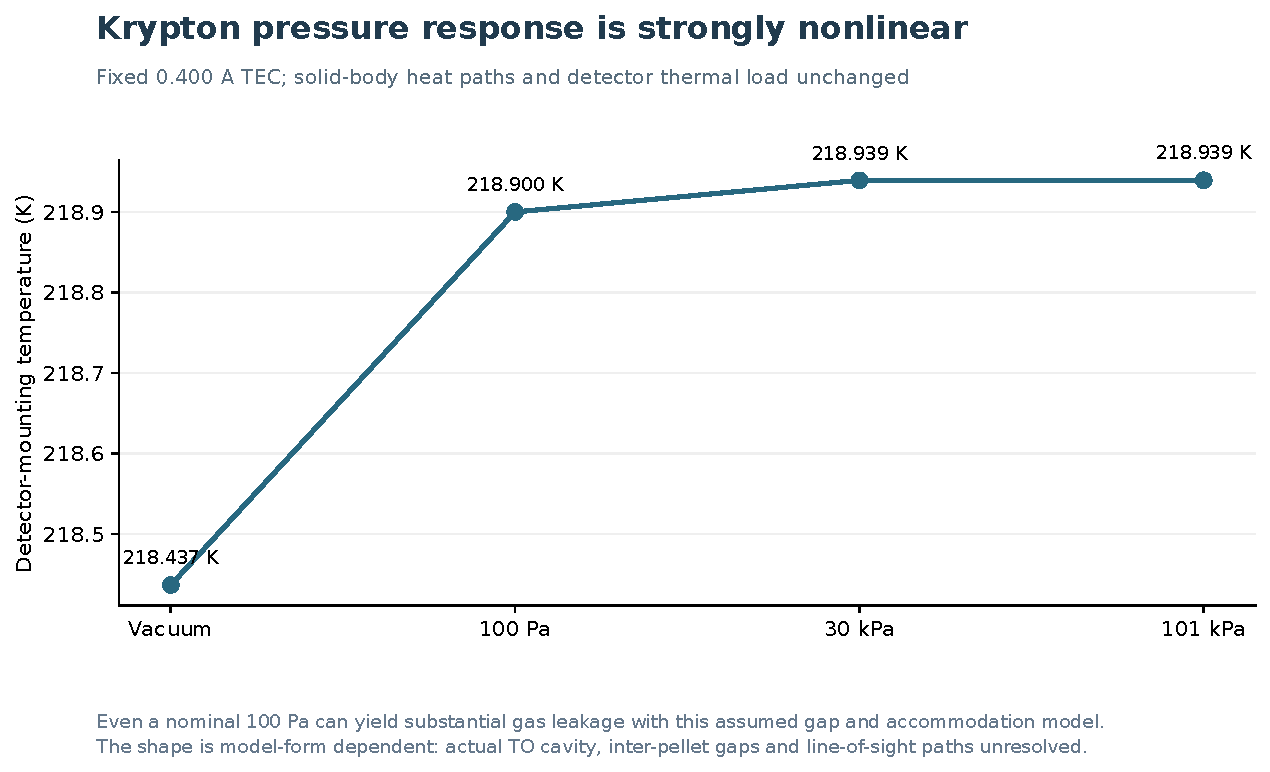
\includegraphics[width=.91\linewidth,height=.42\textheight,keepaspectratio]{figures/v311_krypton_pressure_sensitivity.pdf}
\par\vspace{1mm}{\small\textit{Figure \the\numexpr\value{figure}+1\relax.}
Discrete rarefied-gas/pressure scenarios for Kr in the
declared effective-gap model. Connecting lines are guides only,
not a measured or independently verified continuum response curve.}
\end{center}\stepcounter{figure}

Under this particular model, raising Kr pressure
from 100 Pa to 30 kPa adds just \(0.03930\) K to the device temperature;
raising it from 30 kPa to 101.325 kPa adds only \(0.00010\) K.
This apparent saturation is largely a consequence of the chosen
effective gap, warm-area mapping, and accommodation law.
The physically available narrow gaps between
\(0.40\)-mm-wide pellets spaced on a \(0.58\)-mm pitch
are not represented as independently exposed gas channels.
A more faithful cavity model could change both the pressure
transition and the gas species ranking. The present data
\textbf{must not} be used to claim pressure is unimportant
in an actual TO package at 100 Pa.

\clearpage
\section{Thermal loading, electrical demand, and engineering optimization}
\label{sec:current-design-optimization}
Changing TEC drive current is not a gas effect, but it sets the
trade-off between cold temperature and electrical power.
A separately solved case at \(I_{\rm TEC}=0.550\) A and
30 kPa Kr, with the same 2 mW die heat and 300 K reservoir, gives
\[
T_{\rm top\ ceramic}=205.931\ {\rm K},\quad
T_{\rm die}=206.032\ {\rm K},\quad
P_{\rm TEC}=1.06462\ {\rm W}.
\]
Relative to 0.400 A at 30 kPa Kr this lowers device
temperature by \(12.908\) K while raising terminal input by
\(0.469\) W. Such a trade-off is useful only when a
real operating envelope and safe current/voltage limits
are independently established.

\subsection{Prioritize physical knobs before creating a broad optimization surface}
The existing new-architecture studies support the following
\emph{engineering experiments}, with their distinction between
real geometric variables and screening assumptions preserved.

\begin{center}\small
\begin{tabularx}{\linewidth}{p{42mm}p{33mm}X}\toprule
Construction or operating knob & Existing conditional effect & Next physical qualification\\\midrule
P/N material transport \(k,S,\rho\) &
\(19.8,\ 13.3,\ 4.75\) K source-factor spans &
Real matched P/N grade and correlated properties\\
External mounting resistance &
+2.96 K at +10 K/W, fixed 0.4 A &
TO contact patch, heat spreader and interface pressure\\
Formed-Cu foil/joint thermal path &
6.276 K for an \emph{extreme} contact hypothesis &
Solder/plating area, Cu bending, electrical resistance and current crowding\\
Gas species, 30 kPa, Kr to N$_2$ &
+0.875 K &
Native cavity exposure and inter-pellet gap distribution\\
Detector prescribed load, 1--6 mW &
About 1.56 K span at 0.4 A &
Define die/power budget, attach and carrier conductivity\\
TEC drive current, 0.4 to 0.55 A at 30 kPa Kr &
\(-12.908\) K at \(+0.469\) W &
Rated current, lifetime and allowable package dissipation\\\bottomrule
\end{tabularx}
\end{center}

A physically credible optimization of top-stage temperature should vary
the pellet area \(A\), height \(L\), stage placement, current and
source-grounded package thermal boundaries \emph{jointly}, subject to
specified electrical and mechanical constraints:
\[
\min\,T_{\rm top}(I,A,L,Q_{\rm die},T_{\rm sink},
R_{\rm mount},p_{\rm gas},\ldots).
\]
A transport-only \(A,L\) sweep can isolate competing
\(R_{\rm leg}\sim \rho L/A\) and \(K_{\rm leg}\sim kA/L\)
effects. It cannot by itself be called a fabricated
pellet-geometry variant: changing width or height also changes
solder pad area, foil contact location, ceramic spacing,
interleg gas gaps and insulation clearance.

\subsection{Evidence quality and outstanding physical work}
All eight gas cases and the material/mounting studies archive
original 88-leg nonlinear states, source native four-ceramic
3D nodal fields, input registrations and independent audits.
The eight gas cases all pass direct independently
reconstructed gas conductance, source Cu/lead Joule,
three-stage and global heat balances; their maximum
global energy residual is below \(2\times10^{-9}\) W.
This demonstrates conservation \emph{of the declared model}.
It does not identify actual P/N pellet batches,
solder thermal impedances, or exposed package gas
paths, nor does it establish a full multi-material
430-domain current and thermal PDE.

The next high-value releases should therefore be:
a source-grounded pellet width/height feasibility screen,
a native exposed-surface cavity network,
and a quantified TO mounting/contact construction
study. For each, report \emph{top ceramic temperature},
die mounting temperature, thermoelectric input,
package rejected heat, and individual component
heat-flow budgets. Semiconductor signal/noise and
photodetection belong to the separate specialist model;
they are not necessary to answer these package
thermal-design questions.
\clearpage

% V3.12 source-based contact and mount evidence. Source report and numerical
% results remain unchanged; figure data from archived accepted source states.
\clearpage
\section{Interstage copper, solder interfaces, and the TO mounting path (V3.12)}
\label{sec:v312-contact-mount}
The interstage metal paths are one of the largest existing construction sensitivities in this source-geometry cooler. At the accepted 0.400~A, 300~K reservoir, 100~Pa krypton, and 2.000~mW imposed device heat reference, the three formed-copper networks 58, 80, and stepped three-foot return~88 are conservative electrical/thermal multiports. Their total signed heat delivered to the hot, middle, and upper ceramics is \(-110.578\), \(+25.487\), and \(+87.173\)~mW, respectively. The sum is \(+2.082\)~mW, equal to the source Cu Joule generation; the 87.173~mW entering the upper ceramic is a \emph{redistributed} parasitic heat flow, not 87.173~mW of extra electric input.

\fig[.88]{v312_source_copper_heat_ledger}{pdf}{Original accepted source-geometry V3.5 native copper multiport heat balance. Negative signed values remove heat from the named ceramic. These three components cannot be added as if they were independent heat sources, and the values are not new fitted operating points.}

The upper stage receives \(+41.058\)~mW from net~80 and \(+46.116\)~mW from the upper foot of the stepped return net~88. In contrast, the four effective cavity gas branches transfer a total \(+3.420\)~mW from 100~Pa Kr and the cavity radiation approximation adds \(+0.563\)~mW, to \emph{several different thermal nodes}. The two copper supply leads exchange \(-11.873\) and \(+1.948\)~mW at separate hotter ceramic landings. These are source-specific heat-port values, not a directly additive thermal-load budget for the detector cold tip.

\subsection{Corrected BiSn foil-foot bondline and contact resistance}
Each formed foil has a CAD section \(0.300\times0.030\)~mm and each source joining foot has contact area \(A_c=0.060\ \mathrm{mm^2}\). Its existing effective thermal areal resistance is the \emph{assumed} \(r''_c=10^{-6}\ \mathrm{m^2 K/W}\). For an ideal, completely wetted single solder layer, the bulk-only limit is
\[
 r''_{\rm bulk}=\frac{t}{k_s},\qquad
 R_{\rm foot,bulk}=\frac{t}{k_s A_c}.
\]
The actual formed-foil source joint is \textbf{Bi57Sn43}, not the Sn95Sb5 used at the different P/N leg interfaces. Indium Corporation lists \(k_s=19\ \mathrm{W/(m K)}\) at 85\,$^\circ$C for the adjacent eutectic Bi58Sn42 (Indalloy~281), used here only as an \emph{alloy-family proxy at a different temperature}, and 61~W/(m K) for counterfactual SAC305. These are bulk-material reference values, \emph{not} qualified low-temperature interface data for this synthetic source. The nominal model resistance equals the ideal BiSn-family proxy bulk resistance of a \textbf{19~micrometre} bondline. By contrast, the earlier extreme \(10^{-4}\ \mathrm{m^2K/W}\) contact hypothesis is bulk-equivalent to \textbf{1.9~mm} of this solder and should not be mistaken for a realistic intact solder-foot tolerance. Real wetting, intermetallic layers, plated-film lateral spreading, and interface conditions remain unresolved. The SAC305 comparison is \emph{counterfactual}, not a claim about the source solder composition.

\begin{center}\small
\begin{tabular}{lrrrr}\toprule
Ideal-bulk solder hypothesis & Bondline (\(\mu\)m) & \(r''\) (\(10^{-6}\) m\(^2\)K/W) & Upper Cu (mW) & \(\Delta Q\) (mW)\\\midrule
BiSn proxy, \(k=19\) & 20 & 1.053 & 86.973 & -0.201\\
BiSn proxy, \(k=19\) & 25 & 1.316 & 85.985 & -1.189\\
BiSn proxy, \(k=19\) & 35 & 1.842 & 84.079 & -3.094\\
SAC305 (alternative), \(k=61\) & 20 & 0.328 & 89.825 & +2.651\\
SAC305 (alternative), \(k=61\) & 35 & 0.574 & 88.835 & +1.662\\\bottomrule
\end{tabular}
\end{center}
\fig[.82]{v312_solder_contact_fixed_field_screen}{pdf}{Source-native ceramic face temperatures are frozen while only the ideal bulk-only solder contact conductance varies. This is a conditional, fixed-field copper-flux screen, not a full-system detector-temperature sweep. All heat inputs are reconstructed from saved data without new FEM solves.}

Under these selected hypotheses, 20--35~micrometre BiSn-family proxy bonds change the source upper-stage Cu heat from 86.973 to 84.079~mW at fixed face temperatures, a 2.894~mW span. The original CAD joining foot is 20~micrometres thick; these larger values are a thickness experiment, not the as-built design. In comparison, the prior 100-fold hypothetical contact resistance produces a 6.276~K \emph{fully coupled} detector-temperature decrease; the latter is an extreme interface-isolation experiment, \emph{not} a manufacturable cooler improvement. Net~58 has source-segment thermal conductance 0.002087~W/K (about 479~K/W along the foil) versus 16.67~K/W per nominal foot, illustrating why ideal solder thickness alone is unlikely to eliminate the formed-Cu bypass.

\subsection{Matched-temperature TO mounting penalty and engineering priorities}
An independently accepted V3.8 finite-mount experiment, using its \emph{own provisional temperature-dependent detector Joule load}, increased external mounting resistance by 5 and 10~K/W \emph{in addition to} the existing 4.8334~K/W source package resistance. At fixed 0.400~A this raised the detector temperature from 218.900~K to 220.393 and 221.856~K. Bringing the detector back to within 0.032~K of the reference required currents of approximately 0.4153 and 0.4332~A and increased TEC terminal input from 0.595668~W to 0.648375 (+8.85\%) and 0.712481~W (+19.61\%). These mounting results must not be conflated with the fixed-2~mW solder screen.

The next physical qualification should therefore investigate \textbf{(1)} actual copper-foil, landed solder, and plated-film three-dimensional spreading with electrical continuity; \textbf{(2)} the installed TO mounting/contact geometry and thermal impedance; and \textbf{(3)} narrow exposed cavity-gas paths before geometry-consistent pellet-height and cross-section design optimization. The material and contact parameter intervals are test hypotheses rather than measured statistical tolerance distributions. Full source/audit hashes, the fixed-face solver, and original figures are available in the dedicated V3.12 technical record and its machine-readable result manifest.\footnote{Technical record: \texttt{docs/V3\_12\_COPPER\_JOINT\_MOUNTING\_EVIDENCE\_20261109.md}. Bulk properties: Indium Corporation, Solder Thermal Interface Materials (Bi58Sn42 Indalloy~281, 85\,$^\circ$C analog) and Indalloy~256 SAC305 preform data.}

\clearpage
\section{Native foil-port qualification and the remaining 3D electrical gate (V3.13)}
\label{sec:v313-native-ports}
The next engineering step is not a blind global remesh. For the three-foot source return net88, the existing 1D/effective-contact thermal multiport can be reduced to an explicit three-port response for ceramic faces 36, 74 and 104. Using the current accepted source geometry and independently archived native ceramic-face temperatures, the conductance law for heat \emph{into} the interstage conductor is
\[
\mathbf Q_{\rm foil}=\mathbf G\mathbf T,\quad
\frac{\mathbf G}{10^{-3}\,\mathrm{W/K}}=\begin{bmatrix}
1.952853&-1.892256&-0.060596\\
-1.892256&3.695323&-1.803067\\
-0.060596&-1.803067&1.863663
\end{bmatrix}.
\]
The exact assembled matrix is symmetric and positive semidefinite, has zero row/column sum to numerical precision, and reconstructs accepted 0.400~A copper interface heat to below \(10^{-11}\)~W. This is a verified \emph{reduced source-geometry port operator}, \textbf{not a 3D FEM measurement of foil/spreading conductance}. The actual thermally active middle landing is retained.

\textbf{Electrical topology requiring prospective correction.} In the historical source-registered 3D net88/lead9 coupon, the middle foil foot (`tab\_joint5`, source Bi57Sn43) is an electrical dead end. The reduced V3.4--V3.12 copper law instead includes all three foil-foot electrical contacts in the through-current resistance and allocates current-driven contact heat to all three. At 0.400~A the middle-foot term corresponds to \(R_{c}=0.000166667\ \Omega\) and \(P_{J}=0.026667\)~mW. Omitting this dead-end electrical term in a prospective new source model must not remove the real middle \emph{thermal} contact. Correcting an isolated series coefficient does not establish a new coupled detector temperature or full-module voltage.

\textbf{Historical 3D stop condition.} The original complete 12-region, 28,691-TET4 net88/lead9 physical coupon's fine P1 solution had a worst independent raw one-sided interfacial current-cut mismatch of \textbf{85.63\%}; the subsequent same-mesh P2 mathematical refinement reduced that mismatch to \textbf{8.10\%}, but still failed 11 of 16 mandatory cuts against the original \textbf{0.1\%} criterion. The P2 electric potential also undershot zero by about \(9.15\times10^{-7}\)~V, outside the \(10^{-8}\)~V bound. Its excellent terminal power conservation does not override those failures. Thus \textbf{electrical Gate B remains FAIL/STOP, and physical thermal Gate C and coupled Joule Gate D remain NOT RUN}. The bounded next attempt should qualify the current field and interface ownership first, then compare a genuinely spatial thermal coupon against the matrix above. The archived source mesh, unsuccessful results and gate thresholds remain unchanged.

\textbf{V3.12 correction notice.} Formed-foil feet are \emph{Bi57Sn43}, not the Sn95Sb5 solder used at other TEC P/N junctions. The preceding contact screen is corrected using a \emph{nearby Bi58Sn42 85~$^\circ$C conductivity as an unvalidated family analog}; the source alloy's low-temperature transport is not qualified. Neither correction changes an accepted full-device operating state. Full source hashes, gate records and implementation notes are in \texttt{docs/V3\_13\_NATIVE\_FOIL\_PORT\_AND\_3D\_GATE\_20261109.md}.

\clearpage
\section{Native electrical-contact spatial resolution: failed P2 qualification (V3.14)}
\label{sec:v314-original-coupon}
The next physical coupon experiment tests whether smaller source-CAD elements materially reduce the original 3D lead9/solder contact-gradient mismatch. The same native net88/lead9 12-region BREP, 11 physical contacts, P87-to-pin9 electrical cuts, assumed NOM material tensors and \(r''_e=10^{-11}\ \Omega\,\mathrm m^2\) were retained. Only the Gmsh maximum element size changed, from \(0.045\) to \(0.035\)~mm. No new physical contact law or geometry was fitted, and the middle Bi57Sn43 foil-foot remains a \emph{thermal} landing but an electrical dead-end. The one preregistered, bounded P2 test used 47,277 TET4 geometric cells and 92,495 separate-material quadratic potential DOFs. An independent no-solve saved-field auditor later reconstructed both one-sided interface and terminal current integrals on all 2,178 registered contact triangles, agreeing with the saved producer at \(4.52\times10^{-13}\) relative. The three internal-plane cuts remain producer-only evidence.

\begin{center}\small
\begin{tabular}{lrrl}\toprule
Registered observable & Prior P2 & New finer P2 & Gate\\\midrule
Original geometric tetrahedra & 28,691 & 47,277 & Same BREP\\
P2 scalar DOFs & 58,993 & 92,495 & Same physical regions\\
Worst raw-current mismatch & 8.0993\% & \textbf{7.0193\%} & \textbf{FAIL} (\(\leq 0.1\%\))\\
Current cuts passing & 5/16 & \textbf{5/16} & \textbf{FAIL} (16/16)\\
Minimum electric potential & \(-9.15\times10^{-7}\) V & \(-5.56\times10^{-7}\) V & \textbf{FAIL} (\(\geq-10^{-8}\) V)\\
Unit-excitation coupon resistance & 0.0295489 \(\Omega\) & 0.0295302 \(\Omega\) & Conditional\\
Relative IV--dissipation mismatch & \(6.34\times10^{-9}\) & \(1.43\times10^{-10}\) & PASS (\(\leq0.5\%\))\\\bottomrule
\end{tabular}
\end{center}

\fig[.93]{v314_all_raw_current_cuts}{pdf}{All sixteen original source-identified raw-gradient electrical current-cut mismatches, using the same physical interfaces and criterion before and after the single geometric mesh-size reduction. Eleven of sixteen still fail. Weak/contact-reaction fluxes do not replace these independently verified one-sided element-gradient fluxes. This is not experimental validation or a full-TEC electrical resistance measurement.}

\clearpage
\clearpage
The worst mismatch decreased about 13.33\% relative, yet remains \textbf{70.19 times above the release threshold}. Nine individual raw-cut errors improved, seven worsened. The finer source mesh also has a remaining 0.989\% volume deficit compared with the registered CAD. More importantly, even though the discretized terminal power balance remains excellent, the source contact/lead9 P2 normal-current gradients are not locally accurate to the original standard.

\textbf{Qualification and decision.} The original 3D electrical Gate B remains \textbf{FAIL/STOP}; thermal Gate C and spatial Joule Gate D remain \textbf{NOT RUN}. No new detector operating point, current rating, copper heat-spreading coefficient or manufacturable geometry optimum follows from this failed local coupon. A future approach would need a new separately preregistered source-contact perimeter discretization/field formulation with independent interface and cut-port verification, not an unsupervised mesh sweep or altered acceptance criteria. The full diagnostic and source hashes are archived in \texttt{docs/V3\_14\_NATIVE\_NET88\_P2\_REFINEMENT\_20261109.md}.

\section{Lead9 contact-perimeter field attribution (V3.15)}
\label{sec:v315-perimeter}
The source-native 3D lead9/solder electrical contacts remain the limiting raw-current-gradient problem even after the separate V3.14 fine-mesh P2 solve. This study uses \emph{only the two archived P2 fields}, their unchanged original 12-region source geometry, and the existing 11 finite-contact ownership rules. No new PDE is assembled or solved. On each physical contact facet the two raw currents come from \(-\boldsymbol\sigma\nabla V\), whereas the distinct finite-contact-law current is evaluated from \((V_1-V_2)/r''_e\) using the saved material-separated quadratic traces. The original contact areal resistivity hypothesis is \(r''_e=10^{-11}\ \Omega\mathrm m^2\), not an OEM measurement.

\fig[.88]{v315_lead9_rim_mismatch}{pdf}{Source-native radial TRI3 centroid study of the solder-side absolute raw-gradient/contact-law mismatch. The annular diagnostic bin \(0.90\leq r/r_{\rm CAD}<1.05\) covers about one-fifth of each registered contact surface. The ordinate is the \emph{fraction of that contact's absolute total mismatch} associated with that radial bin, not the local current or a prediction of a newly modified contact.}

For lead9 to the BiSn land, this outer band contains \textbf{78.01\%} of the earlier P2 solder-side absolute mismatch and \textbf{79.11\%} after refinement; for lead9 to the InSn pin joint the corresponding fractions are \textbf{72.47\%} and \textbf{75.94\%}. The registered rim area fractions remain between 19.2\% and 20.4\%. Meanwhile the full-interface raw-current cut errors reduce from 8.0993\% to 7.0193\% (land) and 6.8529\% to 6.1887\% (pin), still greatly exceeding the unchanged \textbf{0.1\%} release limit.

\textbf{Frozen-field negative control.} A counterfactual that zeroes \emph{all of the existing rim's signed raw-minus-contact-law bias} but leaves the interior solved field unchanged would still yield worst signed-side errors of \textbf{2.123\%} at the land and \textbf{1.304\%} at the pin for the finer P2 solution. The counterfactual is not a PDE solution or error bound for a newly solved field, but establishes that removing the currently observed rim discrepancy \emph{alone} is not sufficient. The original physical electrical Gate B remains \textbf{FAIL/STOP}; thermal Gate C and coupled Joule Gate D remain \textbf{NOT RUN}. Future work should favor a separately registered contact-edge/interface-formulation study with original raw-gradient comparisons rather than a generic mesh-size sweep. The complete numerical decomposition and source hashes are documented in \texttt{docs/V3\_15\_LEAD9\_CONTACT\_PERIMETER\_FIELD\_DIAGNOSIS\_20261110.md}.

\section{Independent finite-contact method benchmark and sharp-edge stress test (V3.16)}
\label{sec:v316-method}
The V3.14/V3.15 studies show that detailed source-native 3D current-gradient/contact-law discrepancies persist near the physical solder-contact perimeter, despite low global power and algebraic residuals. Before further attempts on the full lead9/net88 coupon, a separate \emph{two-dimensional nondimensional} method benchmark was solved with a manufactured exact potential. It is not a substitute for or calibration of the actual three-stage TEC source geometry.

Consider two regions \(\Omega_-=(-1,0)\times(0,1)\), \(\Omega_+=(0,1)\times(0,1)\) with constant conductivities \(\sigma_-=1\), \(\sigma_+=3\), contact resistivity \(r_c=0.2\), and linearly varying prescribed current \(Q(y)=1+0.35(y-0.5)\). For a full-height imperfect electrical contact, the exact harmonic fields are
\[
V_{\pm}(x,y)=-\frac{Q(y)x}{\sigma_{\pm}}+0.2y\pm\frac{r_c Q(y)}{2},\qquad
-\sigma_-\partial_x V_-=-\sigma_+\partial_x V_+=\frac{V_--V_+}{r_c}=Q(y).
\]
The variational interface bilinear form is \(\int_{\Gamma}r_c^{-1}(V_--V_+)(w_--w_+)\,d\Gamma\). Independent raw current gradients were integrated on both material sides; no contact-reaction current was substituted for those gradients. Because the exact solution is bilinear and therefore representable by quadratic triangles, this smooth test yields raw-to-contact integrated relative errors \(\mathcal O(10^{-15})\) on 578- and 2,178-DOF discretizations, with separate conserved bulk and interface dissipation.

A deliberately separate contact-tip stress experiment retains the original outside boundary forcing but restricts the interface to \(0.25\leq y\leq 0.75\), insulating the two remaining central boundary segments. The preceding polynomial is no longer an exact solution. The patch test therefore measures \emph{raw-versus-contact internal disagreement}, not physical or mathematical error versus a qualified exact finite-tip field.

\begin{center}\small
\begin{tabular}{rrrr}\toprule
2D subdivision count & Scalar P2 DOFs & Left raw/contact & Right raw/contact\\\midrule
8 & 578 & 11.87\% & 12.58\%\\
16 & 2,178 & 6.44\% & 6.81\%\\
24 & 4,802 & 4.39\% & 4.64\%\\\bottomrule
\end{tabular}
\end{center}

\fig[.90]{v316_sharp_contact_raw_flux}{pdf}{Two-dimensional dimensionless finite-contact method stress case, with sharply terminated contact region and no exact analytic patch solution. The errors are integrated absolute one-sided raw-current versus weak-contact-law discrepancies, \emph{not} the original source-native signed 3D cut-error norm. The displayed 0.1\% source gate is comparative only.}

The smooth manufactured benchmark verifies the standard symmetric P2 weak-contact operator in an exactly representable case. The strong tip-case discrepancy, despite consistent power closure, shows why source-net88 contact-edge verification requires additional field-resolved numerical work. It does \emph{not} establish a singularity mechanism, certify a new discretization, qualify the existing 3D metal model, or provide a new detector temperature. The original 3D electrical Gate B remains \textbf{FAIL/STOP}; thermal Gate C and Joule Gate D remain \textbf{NOT RUN}. Full benchmark code, exact boundary conditions, error norms, and SHA-traceable results are preserved in \texttt{docs/V3\_16\_INDEPENDENT\_CONTACT\_METHOD\_BENCHMARK\_20261110.md}.

\section{Geometric fidelity and remaining discretization risk}
The first full R3.8 TetGen volume candidate contained 1,043,314 tetrahedra over 430 material regions, with all 320,522 registered facets and 378 finite-contact witnesses retained. R3.9 applied 33,195 conservative 3-to-2 internal connectivity operations and reduced the mesh to 1,010,119 tetrahedra with unchanged original surface facets and regional volumes.
\fig[.91]{mesh_quality}{pdf}{Independent archived global mesh-quality measurements. The 3-to-2 flips improved the poor-cell population, but the minimum quality and remaining weak cells prevent assuming mesh-converged coupled FEM.}
R3.9 retains 241,754 tetrahedra with mean-ratio quality below 0.05 (23.93 percent) and a minimum of \(1.38495\times10^{-4}\). Thus no global coupled 430-domain electrical and thermal PDE is released. Historical full-solid electrical Gate B is FAIL/STOP; the first source N/P pair had eight raw gradient-current failures; the prospective P2 and global C/D computations are not qualified. Good energy closure in a separate hybrid model does not erase these original raw gates.

\section{Predicted detector temperature under enclosure loading}
The following \textbf{historical baseline} V3.2 versus V3.3 comparison (prior to adding V3.4 interstage copper) uses the same 88-leg source geometry, 11,791 ceramic tetrahedra, 0.4 A input, 300 K reservoir, 2 mW detector load and assumed material/contact parameters. The cavity raises die temperature \(0.637233\) K, while the nonlinear terminal voltage changes slightly due to changed operating gradients.
\begin{center}\small\begin{tabular}{lrr}\toprule
Metric & V3.2 (cavity off) & V3.3 (cavity on)\\\midrule
\operatingrows
\bottomrule\end{tabular}\end{center}
\fig[.92]{v33_versions}{pdf}{Recorded V1 to V3.3 complete reference-model milestones, all evaluated at the nominal current. These points describe changing model fidelity, not successive mesh convergence or independent measurements.}

\section{Historical V3.3 stage temperatures, heat flow, and electrical input}
\begin{center}\small\begin{tabular}{rrrrrr}\toprule
Stage & Legs & Cold flux (mW) & Hot flux (mW) & V & Joule (mW)\\\midrule
\stagebudgetrows
\bottomrule\end{tabular}\end{center}
\begin{center}\small\begin{tabular}{lr}\toprule Coupled node & Temperature (K)\\\midrule
\nodetablerows
\bottomrule\end{tabular}\end{center}
The external terminal voltage includes additional lead and joint contributions beyond summed P/N voltage. Stage energies must account for signed electrical work, source losses, detector heat, cavity sources and external sink. Directly adding cavity milliwatts to input electrical power without solving the changed stage temperatures would be incorrect.
\fig[.92]{v33_leg_budgets}{pdf}{Real saved individual-leg cold-side heat and terminal-voltage contributions. Stage transitions occur after source leg indices 57 and 79. Source material laws and local ceramic pad temperatures determine leg-specific behavior.}

\section{Historical V3.3 energy conservation and numerical credibility}
For the \textbf{earlier V3.3 baseline only}, the solver used the previous V3.2 solution as a warm start and iterated five spatial leg/pad updates, stopping at a maximum pad temperature change \(1.65345\times10^{-5}\) K below its registered \(2\times10^{-5}\) K criterion. That number is a \emph{numerical stopping threshold}, not a temperature accuracy bound.
\fig[.90]{v33_iterations}{pdf}{Actual saved spatial fixed-point iteration changes and detector temperature history. The last update meets the registered coarse convergence threshold; no mesh refinement or material uncertainty bound is inferred.}
\begin{center}\scriptsize\begin{tabular}{rrrr}\toprule
Iteration & Die T (K) & Max pad update (K) & Local flux mismatch (W)\\\midrule
\iterationrows
\bottomrule\end{tabular}\end{center}
\begin{center}\small\begin{tabular}{lrl}\toprule Metric & Absolute residual & Unit\\\midrule
\residualrows
\bottomrule\end{tabular}\end{center}
An independent read-only field/load audit reconstructs the saved energy terms without rerunning the original PDE and finds a finite \(2.535\times10^{-8}\) W pad/leg update discrepancy. Numerical closure validates the \emph{declared equations and discretization bookkeeping} at this operating point, not prediction fidelity of the as-built cooler.
\section{Device engineering implications and next experiment}
The physical cooler is now represented by a functioning complete thermal/electrical model including a first conservative three-branch copper network tied to original ceramic pads. The present V3.5 corrected-power-lead reference gives 218.900 K (versus V3.4 218.833 K and earlier V3.3 210.625 K); these are conditional modeled values, not manufactured device temperatures. It is \emph{not} necessary to restart cooler CAD development. However, full three-dimensional copper/metal fields and actual thermal-contact characterization are not yet available.
The current and detector-heat-load operating envelope now exists as the accepted V3.6 extension above. The next practical milestone is to couple bounded HgCdTe photoconductor resistance and bias/optical dissipation to that solved thermal environment, while quantifying uncertainty in the \emph{already integrated} multiport: copper conductivity/resistivity versus temperature, joint thermal/electrical impedances, foil thickness and metal-film heat spreading. Use targeted source-informed screening to select conditions that merit expensive full-system recomputation. Full 3D copper FEM may be justified if compact validated metal substructures cannot bound current crowding or nonlocal heat flow.
The older 38-page Revision 3 is preserved because of its unusually useful FEM methodology and publication-level plots, \emph{not} because it describes the current metal layout. The 43-page interim extension is historical, not the latest design reference.

\section{Model provenance and numerical evidence hierarchy}
\begin{tabularx}{\linewidth}{p{30mm}p{37mm}X}\toprule
Artifact & Subject & Verified status\\\midrule
Historical Rev3 & Earlier 216-solid 28/12/4 cooler & Detailed field method; raw-gradient release failed\\
Replacement V3 R1 & 824 physical STEP bodies, formed tabs and joints & Conditional CAD design acceptance\\
R3.9 geometry & 430 material regions, 2,440 CAD faces & Geometric mesh audit; conditioning unqualified\\
V3.3 thermal baseline & 88 nonlinear legs and four source 3D ceramic fields & Accepted reference without formed Cu network\\
V3.4 coupled source Cu & Source ceramics plus formed Cu multiport & Archived accepted reference; combined power-lead heat\\
V3.5 separated TEC leads & Source-local pin 1/9 wire heat and joint sensitivity & Three accepted conditional results; original 3D metal PDE still unqualified\\\bottomrule\end{tabularx}

The cooler envelope is informed by TEC Microsystems MC04 family reference geometry; the package by a separate VIGO nine-pin TO-66 drawing. They are not identified as a commercially fabricated composite. The 29/11/4 stage split, material grades, solder properties and fabricated metal details are source-inspired or chosen synthetic hypotheses, \emph{not} proprietary OEM internals.
\clearpage
\section{Physical assumptions and reproducibility specification}
An independent implementation should use the four 0.5 mm-thick 6.4/5.2/3.8/2.4 mm ceramics, the Appendix B 88 leg centers and polarities, the 29/11/4-couple electrical series order and the source-selected 0.4 by 0.4 by 0.5 mm P/N geometry. Apply all six 14-knot P/N research-material curves in Appendix A; interpolate within the experimental range and explicitly impose the unmeasured quarter-final-segment-slope continuation above 300 K.
Solve 88 individually signed 32-interval nonlinear axial thermoelectric legs and four source-geometry P1 ceramic steady conduction systems using local native TRI3 heat-face integrals. Set the declared assumed ceramic conductivity to 30 W/(m K), add the nominal 176 SnSb joints and 352 assumed electrical contacts, Cu and Au external leads, 2 mW detector heat, the stated finite mounting resistance and the effective 100 Pa Kr/gray radiation closure. For V3.5, include distinct pin1/9 supply lead heat on faces 8 and 36, then include the three finite-contact Cu-foil connections from native faces 38/75, 79/105 and 36/74/104 and iterate to a maximum local pad change below 0.0000003 K and independently check all signed stage and total heat balances.
The archived Appendix C face centroids, areas and flux totals permit a comparable heat-integral replication, not byte-exact nodal temperatures. Bitwise reproduction requires original tetrahedral connectivity, exact face polygon vertices, quadrature and solver conventions. No unpublished real-world detector measurements are claimed.
\section{Scientific and engineering references}
\begin{enumerate}
\item TEC Microsystems, three-stage 3MC04-044-05 cooler family datasheet (2019), external envelope and thermoelectric reference. Its hidden internal routing is unknown.
\item VIGO Photonics, 3TE TO-66 nine-pin housing reference, Rev. 9 (2024). The cooler and housing are independent reference products.
\item J. Zhang et al., low-temperature bismuth telluride thermoelectric measurement and error-analysis study, \emph{Chinese Physics Letters} 42, 056304 (2025). DOI \href{https://doi.org/10.1088/0256-307X/42/5/056304}{10.1088/0256-307X/42/5/056304}. Source P-HE and N-HE-1 specimens are not the actual installed module.
\item M. L. Huber, gas thermal conductivity tabulations (NIST/CRC, 2019): krypton material reference, not experimentally measured gap conduction.
\item TEC Microsystems and Kryotherm multistage construction drawings and photographs; Coherent mounting guidelines. These establish process families, not qualification of the selected synthetic formed-tab design.
\end{enumerate}
\clearpage
\appendix
\section{Complete 14-knot P and N transport source tables}
The following 84 values comprise six figure-digitized research-specimen curves. They do not establish actual commercial material properties. The assumed extension beyond 300 K is
\[
f(T)=f(300)+0.25\,(T-300)\frac{f(300)-f(280)}{20},
\qquad f\in\{S,\rho,k\}.
\]
{\scriptsize\setlength{\tabcolsep}{2.5pt}
\begin{center}\begin{tabular}{rrrrrrr}\toprule
\(T\) K & \(S_P\) & \(\rho_P\) & \(k_P\) & \(S_N\) & \(\rho_N\) & \(k_N\)\\
 & \(\mu{\rm V/K}\) & \(\mu\Omega\,{\rm m}\) & W/(m K) & \(\mu{\rm V/K}\) & \(\mu\Omega\,{\rm m}\) & W/(m K)\\\midrule
\materialrows
\bottomrule\end{tabular}\end{center}}
\clearpage
\section{All original 88 P/N leg centers}
Each leg has 0.1600 mm$^2$ area and 0.5000 mm axial length; stage index 0 is the hottest. All coordinates refer to the original selected synthetic CAD x/y frame in mm.
{\scriptsize\setlength{\tabcolsep}{2.5pt}\renewcommand{\arraystretch}{1.02}
\begin{center}
\begin{tabular}{rrrrr@{\hspace{7mm}}rrrrr}\toprule
No. & Stage & P/N & \(x\) (mm) & \(y\) (mm) &
No. & Stage & P/N & \(x\) (mm) & \(y\) (mm)\\\midrule
\legpairrows
\bottomrule\end{tabular}
\end{center}}
\clearpage
\section{Native ceramic-face geometric and solved heat ledger}
For each original ceramic and native thermal face, the table lists source face ID, centroid (mm), original CAD area (mm$^2$) and the signed integrated solved heat \emph{into} that ceramic (W). Contributions include local P/N transport, provisional joint heating, finite sink, detector and effective cavity loads when applicable. Exact face polygons are not fully specified by centroids and areas.
{\scriptsize\setlength{\tabcolsep}{2pt}\renewcommand{\arraystretch}{1.06}
\begin{longtable}{rrrrrrr}\toprule
Cer. & Face ID & \(x\) & \(y\) & \(z\) & Area mm$^2$ & Heat in (W)\\\midrule\endfirsthead
\toprule Cer. & Face ID & \(x\) & \(y\) & \(z\) & Area & Heat (W)\\\midrule\endhead
\padrows
\bottomrule\end{longtable}}
\clearpage
\section{Verification boundaries and remaining work}
\begin{tabularx}{\linewidth}{p{38mm}p{30mm}X}\toprule
Technical claim & Actual status & Appropriate requirement for improvement\\\midrule
824-solid replacement V3 CAD & Conditional physical-design PASS & Measured forming, solder, current and reliability capability\\
Native pin-to-pin topology & 88/88 legs PASS & Finite real current density, resistance and contact temperature fields\\
Global 430-domain R3.9 mesh & Geometric PASS & Improve worst elements and prove solver conditioning/convergence\\
Original full-solid electrical Gate B & Historical FAIL/STOP & Qualify original raw-gradient tests on a viable mesh\\
Full 430-domain electrothermal PDE & NOT RUN & Integrated metal/contact/leg/ceramic field solution\\
V3.5 Cu and source-lead hybrid at 0.4 A & Conditional numerical PASS & Solder/foil interface and plated metal-sheet laws, then current/load response\\
Rarefied gas and radiation & Effective load model & Native exposed-surface gas/gray/spectral physics\\
Real thermoelectric grades & Unidentified & Bounded synthetic studies or actual module certificates\\
HgCdTe photodetection & No carrier/optical PDE & Detector noise/spectral/bias physics if needed\\
As-built product prediction & Unvalidated & Device measurements; do not claim manufacturer equivalence\\\bottomrule
\end{tabularx}
\vspace{5mm}

{\color{navy}\rule{\linewidth}{1pt}}

{\small\textbf{Publication policy.} The original 38-page Revision 3 remains a sealed separate historical methodology reference. Its later 43-page interim source-mesh integration is likewise archived. This document describes the newer replacement CAD and the most recent completed running hybrid with the unmodeled internal copper paths prominently disclosed. All figures and numerical tables derive from existing saved evidence, and no new physics calculation was performed for this publication.}
\end{document}
